\documentclass[12pt,times,oneside,openright,hardcopy]{eeereport}
\renewcommand{\baselinestretch}{1.08}

\usepackage{amsmath}
\usepackage{amssymb}
\usepackage{booktabs}
\usepackage{multirow}
\usepackage{array}
\usepackage{tabularx}
\usepackage{siunitx}
\usepackage{xcolor}
\usepackage{listings}
\usepackage{algorithm}
\usepackage{algpseudocode}
\usepackage{placeins}
\usepackage{caption}
\usepackage{etoolbox}
\usepackage{makecell}
\usepackage{pifont}
\usepackage[hidelinks]{hyperref}
\usepackage{microtype}
\usepackage{enumitem}

\renewcommand{\arraystretch}{1.02}
\newcolumntype{Y}{>{\raggedright\arraybackslash}X}
\newcolumntype{C}{>{\centering\arraybackslash}X}
\newcolumntype{L}[1]{>{\raggedright\arraybackslash}p{#1}}
\newcolumntype{R}[1]{>{\raggedleft\arraybackslash}p{#1}}
\captionsetup{font=small,labelfont=bf,skip=2pt}
\captionsetup[figure]{font=small,labelfont=bf,skip=2pt}
\captionsetup[table]{font=small,labelfont=bf,skip=1pt}
\newcommand{\compacttable}{\small\renewcommand{\arraystretch}{0.90}\setlength{\tabcolsep}{1.60pt}}
\newcommand{\tighttable}{\footnotesize\renewcommand{\arraystretch}{0.86}\setlength{\tabcolsep}{1.15pt}}
\newcommand{\lookuptable}{\scriptsize\renewcommand{\arraystretch}{0.84}\setlength{\tabcolsep}{0.95pt}}
\AtBeginEnvironment{algorithmic}{\scriptsize}
\floatstyle{ruled}
\restylefloat{algorithm}
\setlength{\textfloatsep}{5pt plus 1pt minus 1pt}
\setlength{\floatsep}{4pt plus 1pt minus 1pt}
\setlength{\intextsep}{4pt plus 1pt minus 1pt}
\renewcommand{\topfraction}{0.92}
\renewcommand{\bottomfraction}{0.82}
\renewcommand{\textfraction}{0.06}
\renewcommand{\floatpagefraction}{0.86}
\setlist[itemize]{leftmargin=*, itemsep=1.5pt, topsep=2pt}
\setlist[enumerate]{leftmargin=*, itemsep=1.5pt, topsep=2pt}
\sisetup{detect-all=true}
\renewcommand{\bibname}{References}
\makeatletter
\let\watermarkscope@addcontentsline\addcontentsline
\newcommand{\suppressappendixsubtoc}{%
  \renewcommand{\addcontentsline}[3]{%
    \def\watermarkscope@toclevel{##2}%
    \def\watermarkscope@section{section}%
    \def\watermarkscope@subsection{subsection}%
    \def\watermarkscope@subsubsection{subsubsection}%
    \ifx\watermarkscope@toclevel\watermarkscope@section
    \else\ifx\watermarkscope@toclevel\watermarkscope@subsection
    \else\ifx\watermarkscope@toclevel\watermarkscope@subsubsection
    \else
      \watermarkscope@addcontentsline{##1}{##2}{##3}%
    \fi\fi\fi
  }%
}
\newcommand{\appendixchapter}[2]{%
  \cleardoublepage
  \refstepcounter{chapter}%
  \setcounter{section}{0}%
  \chapter*{Appendix \thechapter\\#1}%
  \phantomsection
  \watermarkscope@addcontentsline{toc}{section}{Appendix \thechapter: #1}%
  \markboth{Appendix \thechapter. #1}{Appendix \thechapter. #1}%
  \label{#2}%
}
\makeatother
\newcommand{\claimrow}{\ensuremath{\mathsf{row}}}
\newcommand{\claimbearing}{\ensuremath{\mathsf{claim}}}
\newcommand{\supportonly}{\ensuremath{\mathsf{support}}}
\newcommand{\needsreview}{\ensuremath{\mathsf{needs\_review}}}
\newcommand{\artifact}[1]{\textnormal{\small #1}}
\newcommand{\stagebullet}{\textcolor{black!70}{\ding{117}}}
\newcommand{\claimmark}{\textcolor{black!70}{\ding{72}}}
\newcommand{\insightbox}[1]{%
  \begin{center}
  \setlength{\fboxsep}{6pt}%
  \fcolorbox{black!20}{black!3}{%
    \begin{minipage}{0.91\textwidth}
    \small\itshape #1
    \end{minipage}}%
  \end{center}}
\newcommand{\questionbox}[1]{%
  \begin{center}
  \setlength{\fboxsep}{5pt}%
  \fcolorbox{black!18}{black!3}{%
    \begin{minipage}{0.88\textwidth}
    \centering\small\textbf{\emph{#1}}
    \end{minipage}}%
  \end{center}}

\lstset{
  basicstyle=\ttfamily\footnotesize,
  breaklines=true,
  frame=lines,
  rulecolor=\color{black!25},
  backgroundcolor=\color{black!2},
  numbers=none,
  captionpos=b,
  showstringspaces=false,
  columns=fullflexible,
  keepspaces=true
}

\begin{document}
\linespread{1.08}
\pagenumbering{Alph}

\begin{titlepage}
  \begin{center}
    
\includegraphics[scale=0.5]{fig/xjtlu_logo_blue.pdf}\\[0.3in]
    \large \textbf{DTS311TC Final Year Project}\\[0.2in]
    \huge \textit{\textbf{WatermarkScope: A Benchmark-to-Audit Framework for Source-Code Watermarking in Code Generation Models}}\\[2.0in]
    \normalsize
    \small \textbf{In Partial Fulfillment of \\ the Requirements for the Degree of \\ Bachelor of Engineering} \\[0.3in]
    \normalsize
    By \\
    \textbf{Haoyi Zhang}\\
    Student ID: \textbf{2254912} \\
    \vspace{.2in}
    Supervisor\\
    {\textbf{Md Maruf Hasan}}\\[0.1in]
    \vfill
    {School of AI and Advanced Computing}\\
    \normalsize
    \textsc{Xi'an Jiaotong-Liverpool University}\\
    May 2026
  \end{center}
\end{titlepage}

\frontmatter

\chapter{Abstract}
Large language models increasingly generate source code that is copied, edited, translated, and deployed outside the original generation session. This project presents \emph{WatermarkScope}, a benchmark-to-audit framework for evaluating source-code watermarking evidence under realistic code-generation conditions. The framework connects five stages: CodeMarkBench defines executable benchmark denominators; SemCodebook studies structured white-box provenance recovery; CodeDye preserves conservative black-box null-audit evidence; ProbeTrace evaluates scoped active-owner attribution; and SealAudit examines marker-hidden security triage. The current evidence surface includes 140/140 canonical CodeMarkBench runs, 23,342/24,000 SemCodebook recoveries with 0/48,000 negative-control hits, 6/300 CodeDye sparse live signals with 170/300 positive controls and 0/300 negative controls, 300/300 ProbeTrace scoped decisions with 0/1,200 false-owner controls, and 81/960 decisive SealAudit triage outcomes with 0 observed unsafe passes. The main conclusion is that source-code watermarking should not be judged by one detector score. Reliable evaluation requires fixed denominators, executable controls, uncertainty reporting, access-specific claim boundaries, and explicit abstention when evidence is insufficient.

\par\vspace{0.28em}\noindent\textbf{Keywords:}\\
Watermark Evidence; Executable Evaluation; Provenance Recovery; Owner Attribution; Risk Triage.


\tableofcontents

\mainmatter
\pagenumbering{arabic}

\chapter{Introduction}\label{cpt:intro}

Large language models for code generation have moved from laboratory demonstrations to everyday software engineering workflows~\cite{chen2021codex,roziere2023codellama}. Models trained or aligned for programming tasks can produce functions, scripts, tests, data-processing pipelines, and repository patches from natural-language prompts. Their outputs are not static text artifacts: they are compiled, executed, reformatted, translated between languages, edited by humans, and incorporated into larger systems. This property makes provenance and watermarking for generated code both important and technically difficult. A watermark that is visible only in a surface string may disappear after a normal refactoring; a detector that ignores program semantics may flag harmless controls; and a provenance method that damages executable behavior is unlikely to be useful in practice~\cite{kirchenbauer2023watermark,li2023protecting,lee2024who}.

This dissertation is organized around one research question:

\questionbox{How can source-code watermarking be evaluated, embedded, traced, and audited under realistic code-generation conditions?}

The answer developed here is \emph{WatermarkScope}, a benchmark-to-audit framework. I do not treat watermarking as a single binary detector, because the meaning of a detector hit changes with access to the model, the available artifacts, and the risk question being asked. WatermarkScope therefore follows a staged argument. It begins with an executable benchmark for existing runtime watermarking methods, then introduces a structured white-box provenance watermark, and finally moves into black-box null audit, active source attribution, and security triage. In this sequence, \emph{evaluated} maps to CodeMarkBench, \emph{embedded} to SemCodebook, \emph{traced} to CodeDye and ProbeTrace, and \emph{audited} to SealAudit. The ordering matters: fragile benchmark behavior motivates structured provenance; black-box deployment requires a weaker but auditable record; ownership claims require a fixed active-owner registry; and security-sensitive markers require selective review rather than automatic acceptance.

The organizing principle is an \emph{evidence contract}. Each module has to say what kind of observation it produces, which denominator that observation belongs to, and which interpretation it does not support. This is what keeps the dissertation from becoming five unrelated result tables. Formally, a stage is summarized as
\begin{equation}
  \mathcal{L}_j =
  (\mathcal{A}_j,\mathcal{O}_j,\mathcal{D}_j,\mathcal{C}_j,\delta_j,\mathcal{M}_j,\mathcal{I}_j,\mathcal{F}_j),
  \label{eq:lifecycle-stage}
\end{equation}
where $j\in\{\mathrm{benchmark},\mathrm{provenance},\mathrm{audit},\mathrm{attribution},\mathrm{triage}\}$, $\mathcal{A}_j$ is the access model, $\mathcal{O}_j$ is the evidence object, $\mathcal{D}_j$ is the fixed denominator, $\mathcal{C}_j$ is the control set, $\delta_j$ is the frozen decision rule, $\mathcal{M}_j$ is the reported metric vector, $\mathcal{I}_j$ is the allowed interpretation, and $\mathcal{F}_j$ is the set of forbidden interpretations. The lifecycle advances only when $\mathcal{A}_j$ or the risk question changes enough that the previous evidence object cannot support the next claim. This is the main reason CodeDye, ProbeTrace, and SealAudit are not weaker versions of SemCodebook; they answer different evidence questions under different access contracts.

For example, a detector hit in CodeMarkBench is not automatically provenance, contamination evidence, ownership evidence, or safety evidence. It becomes a SemCodebook provenance claim only when the structured carrier and recovery contract is available; it becomes a CodeDye audit signal only when the transcript-bound black-box predicates are frozen; and it becomes a ProbeTrace attribution only under a registered active owner. The same observation therefore changes meaning as the access model changes.

This formalization is stricter than a normal project summary, but the extra discipline is useful. The decision rule $\delta_j$ must be fixed before the result is interpreted; otherwise a later threshold change could turn a diagnostic artifact into an attractive claim. The metric vector $\mathcal{M}_j$ is reported instead of a single portfolio score because recovery, audit yield, attribution, and triage coverage are not the same event. The forbidden set $\mathcal{F}_j$ is also part of the method: a numerical result can look strong and still be scientifically weak if the writing invites a deployment claim that the evidence does not support.

\insightbox{A WatermarkScope result is not just a detector firing. It is a detector output plus an access model, a fixed denominator, a control surface, and a forbidden-claim boundary.}

The five projects are therefore not separate endpoints. Each stage begins where the previous evidence object stops being sufficient: executable benchmarking establishes the denominator, structured carriers support white-box provenance, transcript preservation supports black-box audit, owner registries support scoped attribution, and marker-hidden triage handles security risk. The dissertation's story is the movement from executable evidence to deployable evidence under weaker access and higher governance risk.

\section{Motivation}

Watermarking for ordinary natural language is often evaluated by measuring whether a detector can distinguish generated text from human text under paraphrasing or sampling changes~\cite{kirchenbauer2023watermark,zhao2024provable}. Source code adds several additional constraints. First, generated code has executable semantics: a method that leaves a detectable signal but breaks tests has not solved the practical problem. Second, transformations such as identifier renaming, comment removal, control-flow rewriting, helper extraction, formatting, translation, and dependency repair are normal software operations rather than adversarial edge cases. Third, code-generation systems are often accessed through heterogeneous interfaces: local white-box models, cloud APIs, private fine-tuned students, and benchmark pipelines. Finally, code is security-sensitive. A watermark, marker, or audit prompt may interact with unsafe code patterns, hidden triggers, or provider-level moderation decisions~\cite{pearce2022asleep,perry2023users,siddiq2023llmseceval}.

These constraints motivate a broader evaluation stance. The dissertation asks not only whether a detector fires, but also what denominator it fires on, whether controls remain clean, whether evidence is claim-bearing or support-only, whether uncertainty is reported, and whether the system abstains when evidence is insufficient. This is especially important for avoiding overclaiming. A sparse black-box signal is not a prevalence estimate. A perfect attribution result in one owner setting is not provider-general authorship proof. A selective triage system with high abstention is not an automatic safety classifier.

\section{Design Objectives}

The framework is built around four design objectives. First, results must be executable: a watermark result is not useful if the generated code cannot pass the intended tests. Second, evidence must be denominator-aware: every reported rate must have a fixed claim-bearing denominator and a clear treatment of support-only rows. Third, controls must be explicit: negative controls, false-owner controls, and marker-hidden controls are reported as first-class results rather than buried in implementation notes. Fourth, the system must be allowed to abstain when evidence is insufficient. These objectives are closer to an engineering audit discipline than to a single classifier benchmark.

\section{Lifecycle Framing}

Table~\ref{tab:intro-lifecycle} summarizes how the five stages connect. The important point is that the access model changes across the lifecycle. A white-box provenance method can make stronger claims than a black-box audit, but only within admitted model cells. An active-owner attribution protocol can make stronger source claims than a passive detector, but only after the owner registry is fixed. A safety triage protocol can be useful even with high abstention if it avoids unsafe pass-through. This is why the dissertation reports several evidence surfaces instead of reducing the work to one score.

\begin{table}[htbp]
\centering
\caption{WatermarkScope as one benchmark-to-audit lifecycle.}
\label{tab:intro-lifecycle}
\tighttable
\begin{tabularx}{\textwidth}{@{}L{1.75cm}L{2.15cm}YL{2.35cm}@{}}
\toprule
Stage & Handoff trigger & Evidence object & Claim boundary \\
\midrule
Benchmark & Executability gap & Run inventory and metric vector & Finite release matrix \\
Provenance & Carrier gap & AST/CFG/SSA recovery & Admitted white-box cells \\
Audit & Access gap & Hash-bound transcript evidence & Null audit, not prevalence \\
Attribution & Ownership gap & Owner-bound witness record & Single active owner \\
Triage & Safety gap & Marker-hidden triage row & Selective audit \\
\bottomrule
\end{tabularx}
\end{table}

\section{Contributions}

The dissertation makes five connected contributions. These are contribution points along the same evidence chain, not standalone objectives.

\begin{itemize}
  \item[\stagebullet] \textbf{Benchmark contract}: CodeMarkBench provides an executable benchmark foundation with four pinned runtime baselines, five local code models, seven benchmark source groups, and a canonical 140/140 run-completion matrix. The repository entry points are recorded in Appendix~\ref{app:repository-access}.
  \item[\stagebullet] \textbf{White-box provenance}: SemCodebook uses AST, CFG, and SSA carrier families with keyed scheduling and error-correcting recovery for admitted white-box model cells.
  \item[\stagebullet] \textbf{Black-box audit}: CodeDye preserves hash-bound raw-response and structured evidence while refusing to infer contamination prevalence from sparse signals.
  \item[\stagebullet] \textbf{Source attribution}: ProbeTrace uses owner registries, semantic witnesses, decoys, and false-owner controls for active-owner, source-bound attribution.
  \item[\stagebullet] \textbf{Security triage}: SealAudit reports marker-hidden selective triage, explicit needs-review outcomes, and unsafe-pass boundaries.
\end{itemize}

\begin{figure}[!t]
  \centering
  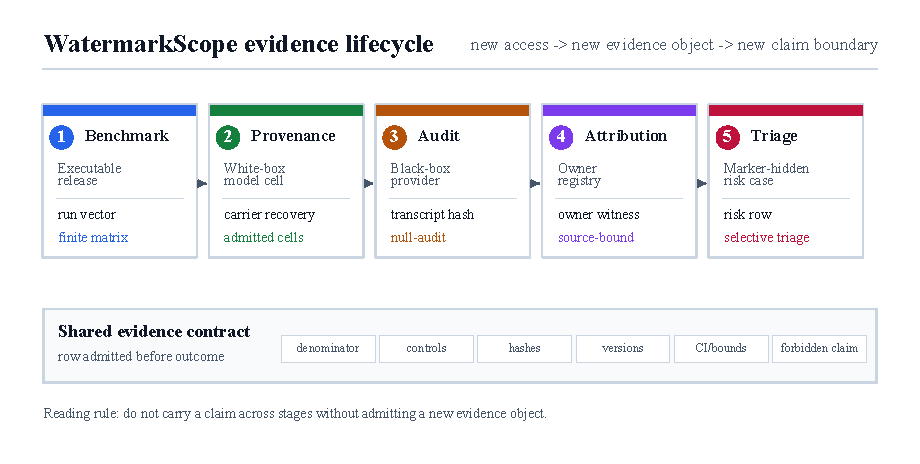
\includegraphics[width=\textwidth]{fig/watermarkscope_framework_map.pdf}
  \caption{WatermarkScope evidence lifecycle. A new access model creates a new evidence object and claim boundary; claims do not transfer across stages without a new admitted surface.}
  \label{fig:watermarkscope-pipeline}
\end{figure}

\section{Threat Model and Evaluation View}

The threat model assumes that generated code may be transformed by normal developer actions or by deliberate laundering attempts. Such transformations include identifier renaming, comment stripping, formatting changes, helper extraction, control-flow rewriting, cross-language translation, and query-budget changes in black-box audits. The defender or auditor may have white-box access to a local model in SemCodebook, black-box transcript access in CodeDye, a registered active-owner key in ProbeTrace, or only marker-hidden audit evidence in SealAudit. The thesis therefore uses different claim types for different access models instead of pretending that one detector can answer all provenance questions.

\section{Scope and Non-Claims}

The dissertation is careful about scope. CodeMarkBench does not prove that all source-code watermarking fails; it evaluates the included runtime baselines under the included models, source groups, and stress conditions. SemCodebook does not claim universal semantic watermarking; it claims structured provenance recovery within admitted white-box family and scale cells. CodeDye does not accuse a model provider of contamination and does not estimate contamination prevalence. ProbeTrace does not claim provider-general or multi-owner attribution. SealAudit does not certify watermark harmlessness or provide an automatic safety classifier. These limits are not apologies for the work. They are the boundaries that make the results checkable.

This scoping also defines how the implementation should be inspected. The submitted WatermarkScope repository is the FYP artifact: it contains the dissertation source, method snapshots, result manifests, preserved evidence summaries, and examiner-facing verification scripts. CodeMarkBench is separately listed because it is an earlier benchmark artifact that supplies the executable foundation for the first stage. It should be read as supporting infrastructure for the lifecycle, not as a second dissertation. Appendix~\ref{app:repository-access} lists both access points and explains which repository should be used for marking.

The distinction matters for assessment. A design project is not complete when a PDF describes an idea; it must expose enough implementation structure for an examiner to inspect how the evidence was generated, which files bind to the printed claims, and which checks can be rerun without private keys or GPUs. For this reason, the report treats code and manifests as part of the argument rather than as optional supplementary material. The writing names the evidence surfaces, but the repository supplies the artifact paths, hashes, and scripts that make those surfaces auditable.

The remaining chapters follow the same lifecycle order: background, executable benchmark foundation, white-box and black-box evidence protocols, attribution and security triage, and finally a synthesis of confidence intervals, claim boundaries, and future work. This order is part of the argument. Each chapter changes the evidence object only when the previous access model can no longer support the next claim, and the report avoids a single portfolio score because recovery, audit yield, attribution, and triage coverage are different events rather than interchangeable measurements.

The reader should therefore track two threads at the same time. The first thread is technical: how to build benchmark rows, structured carriers, transcript-bound audit records, owner witnesses, and marker-hidden triage rows. The second thread is evidential: how each row becomes admissible, which denominator it enters, and which interpretation is deliberately blocked. A strong result in this dissertation is not simply the largest numerator. It is a result whose numerator is tied to a stable denominator, whose controls make the failure modes visible, and whose wording does not move beyond the access model that produced the evidence. The following chapter therefore reviews benchmarks, watermarking, provenance, and security as evidence problems rather than as isolated literatures.

This reading lens is also the standard used to judge the submitted design artifact. A technically strong implementation is not enough if the written claim moves faster than the evidence; a carefully scoped claim is not enough if the repository cannot show how the row was produced. WatermarkScope is intended to satisfy both requirements at once. The chapters therefore alternate between method design and evidence accounting: each protocol is introduced through the access assumption that makes it possible, the records that make it auditable, and the boundary that stops it from becoming a broader claim than the experiment supports.

This also explains the report's treatment of negative results and abstentions. The benchmark chapter does not hide baseline tradeoffs; the white-box chapter keeps misses inside the recovery denominator; the black-box chapter reports sparse signals as sparse; the attribution chapter writes a perfect scoped result as scoped; and the triage chapter treats review load as an outcome rather than a nuisance. These choices make the dissertation less sensational, but they make it more inspectable. A reader should be able to ask, for every number in the report, four questions: what was counted, what was excluded before the outcome was known, what control surface was used, and what conclusion is forbidden. The rest of the dissertation is organized to answer those questions in the same order as the lifecycle.

\chapter{Background and Related Work}\label{cpt:background}

This chapter positions the dissertation within four bodies of work: code-generation models and executable benchmarks, watermarking for generated text and code, data provenance and contamination analysis, and security evaluation for generated code. The purpose is not to survey every paper in these areas. Instead, the chapter identifies the assumptions that motivate WatermarkScope's design: code artifacts must execute, benchmark claims need stable denominators, watermark detection needs negative controls, and security-sensitive systems need abstention rather than forced decisions.

\section{Code Generation Models}

Large language models trained on code have made program synthesis a practical research area. Earlier neural code models such as CodeBERT, PLBART, and CodeT5 established reusable code representations and sequence-to-sequence pre-training for program understanding and generation~\cite{feng2020codebert,ahmad2021plbart,wang2021codet5}. Codex and HumanEval then established pass@k-style functional evaluation for generated Python programs~\cite{chen2021codex}. Later generative code models such as InCoder and Code Llama broadened the setting to infilling, editing, and local open-model evaluation~\cite{fried2023incoder,roziere2023codellama}. These developments motivate this dissertation's model setting: source-code watermarking should be evaluated on executable model outputs, not only on token streams.

The executable nature of code changes the meaning of watermark quality. A generated answer can carry a watermark while failing tests, or pass tests while losing the watermark after ordinary edits. A useful evaluation must therefore track both evidence quality and program utility. This principle appears throughout CodeMarkBench and the later protocol modules.

\section{Executable Code Benchmarks}

Code evaluation benchmarks differ in scope. CodeXGLUE aggregates a broad set of code understanding and generation tasks~\cite{lu2021codexglue}. MBPP focuses on short Python programming problems~\cite{austin2021mbpp}, while APPS introduces competition-style programming tasks with larger solution spaces~\cite{hendrycks2021apps}. MultiPL-E extends code-generation evaluation across programming languages~\cite{cassano2022multiple}. DS-1000 emphasizes data-science code and highlights the difficulty of contamination-aware evaluation~\cite{lai2023ds1000}. SWE-bench moves toward repository-level issue resolution~\cite{jimenez2024swebench}, and LiveCodeBench explicitly targets live benchmark construction to reduce contamination risks~\cite{jain2024livecodebench}. BigCodeBench further broadens execution-based code evaluation to library-rich tasks requiring multiple function calls and complex instructions~\cite{zhuo2025bigcodebench}.

These benchmarks motivate several design decisions in CodeMarkBench. First, one source group is not sufficient; a benchmark should include public and crafted sources. Second, language coverage matters because transformations that preserve Python behavior may not preserve Java, C++, Go, or JavaScript behavior. Third, a benchmark should record exact run identities and release contracts, because later comparisons are meaningful only if the denominator remains stable.

\section{Watermarking Generated Text and Code}

Watermarking for generated text often uses a keyed bias in token selection and a statistical detector over the generated sequence. Kirchenbauer et al. introduced a widely cited green-list watermarking formulation for large language models~\cite{kirchenbauer2023watermark}. Subsequent work studies robustness, reliability, provability, and undetectability under different edit or access assumptions~\cite{zhao2024provable,kirchenbauer2024reliability,christ2024undetectable}. Code watermarking, however, has additional structure. Generated code contains syntax trees, control flow, data flow, dependencies, tests, comments, and naming conventions. Code-oriented watermarking and API watermarking work therefore needs to balance detector strength with executable utility and edit robustness~\cite{li2023protecting,lee2024who,suresh2024robust}.

This dissertation uses prior watermarking work in two ways. CodeMarkBench evaluates existing runtime code-watermarking baselines under a shared release contract whose repository and artifact entry points are recorded in Appendix~\ref{app:repository-access}. SemCodebook then moves away from purely surface-level evidence by treating structured program carriers as recoverable provenance support. This does not make the watermark universal; it makes the claim more explicit about carrier families and admitted model cells.

\section{Why Code Changes the Watermarking Problem}

The difference between text and code watermarking is not only that code has syntax. The deeper issue is that ordinary software maintenance can change the observable surface while preserving the intended behavior. A developer may rename variables, extract a helper, remove comments, normalize formatting, replace an expression with an equivalent library call, or translate a solution into another language. A detector that depends on the original token surface can fail after these edits even when the program remains a legitimate descendant of the generated artifact.

The reverse failure is also possible. A detector can fire on clean code because a formatting style, naming pattern, or common control-flow idiom happens to resemble a watermark carrier. This is especially dangerous for source-code watermarking because false positives can imply authorship, contamination, or security risk. WatermarkScope's design therefore treats negative controls and executable preservation as part of the central evidence, not as a secondary sanity check. A result that has a high detector rate but an unclear control denominator would be weak evidence for this dissertation.

This observation explains why the later modules have different access assumptions. SemCodebook uses structured carriers because white-box access allows the method to inspect program representations rather than only token strings. CodeDye does not attempt the same recovery in a black-box API setting because the necessary carriers and model internals are unavailable. ProbeTrace adds an owner registry because detection is not the same as attribution. SealAudit adds a triage resolver because provenance evidence does not answer whether the watermarking mechanism is safe.

\section{Provenance, Memorization, and Contamination}

Training data extraction and memorization studies show that large language models can reproduce or expose training examples under certain conditions~\cite{carlini2021extracting,carlini2023quantifying}. Membership and pretraining-data detection methods, such as Min-K\% probability approaches, study whether a model has likely seen a candidate sequence~\cite{shi2023detecting}. Benchmark contamination surveys further show that evaluation datasets can leak into pretraining or instruction-tuning corpora, complicating claims about model capability~\cite{xu2024contamination}. Data statements and dataset documentation encourage explicit provenance, collection, and intended-use descriptions~\cite{bender2018data}.

These works motivate CodeDye's conservative framing. A black-box audit may surface sparse evidence, but it should not turn a small signal count into a contamination prevalence estimate. Instead, it should preserve prompt hashes, raw response hashes, structured payload hashes, controls, and threshold versions so that later human or provider-side review can examine the evidence without changing the denominator.

The same provenance literature also clarifies why attribution is not the same as detection. A detector can say that an output resembles a class of examples, while an attribution protocol must bind the output to a registered source or owner under a precommitted rule. ProbeTrace therefore introduces an active owner registry rather than treating high similarity as authorship. This distinction is important for the dissertation story: CodeDye preserves black-box evidence when ownership is unknown, while ProbeTrace studies the stronger but narrower setting where the owner key and source split have already been registered.

\section{Security Evaluation for Generated Code}

Generated-code safety research shows that code assistants can produce insecure code or influence developers toward insecure patterns. Pearce et al. studied insecure code suggestions from GitHub Copilot~\cite{pearce2022asleep}. Perry et al. found that AI assistants can affect whether users write secure or insecure code~\cite{perry2023users}. LLMSecEval provides a dataset for evaluating security properties of LLM-generated code~\cite{siddiq2023llmseceval}. Security taxonomies such as the MITRE CWE Top 25 provide practical categories for common software weaknesses~\cite{mitre2025cwe}.

These studies motivate SealAudit. A watermark or marker should not be treated only as a provenance signal. If a marker changes model behavior, triggers unsafe completions, or interacts with laundering and spoofability attacks, it becomes a security-relevant object. SealAudit therefore reports selective triage with explicit needs-review outcomes rather than claiming that a model is safe.

\section{Gap Addressed by This Dissertation}

The gap is not simply the absence of another detector. The gap is an evidence protocol for deciding what a detector result is allowed to mean. The works reviewed above motivate this point from different directions: code benchmarks emphasize executable evaluation, watermarking papers emphasize keyed detection and robustness, provenance work warns against unsupported data-use inference, and security studies show that generated code can carry deployment risk. WatermarkScope addresses the combined gap by putting benchmark foundation, structured provenance recovery, conservative null-audit, active attribution, and selective triage under one claim-boundary discipline.

A second gap is methodological rather than only empirical. Many watermarking papers optimize a detector score, but a source-code watermarking system also has to specify what counts as a valid observation. A syntactic perturbation that changes the test outcome should not be treated the same as an executable semantic-preserving rewrite. A negative control that lacks the target watermark must be preserved even when it makes the result less impressive. A row generated for debugging, canary checking, or failure localization should not silently enter a main table. This dissertation therefore treats evidence admission as part of the method. The admission rule defines which rows may support a claim before the detector result is known.

The final gap concerns how to compare results across different access assumptions. White-box provenance, black-box null-audit, active-owner attribution, and security triage are not interchangeable tasks. A high recovery rate in an admitted white-box setting does not imply contamination detection in a black-box provider setting. Conversely, a sparse black-box audit signal is not a failed watermark if the stated goal is to preserve auditable evidence under conservative thresholds. The WatermarkScope framing is useful because it makes these access assumptions explicit. Each module reports the strongest claim that its evidence supports, and the dissertation avoids converting one module's metric into another module's conclusion.

These gaps appear sequentially as access changes: benchmark, provenance, audit, attribution, and triage. The rest of the dissertation follows that sequence instead of treating the artifacts as independent endpoints. Code-generation benchmarks contribute executable tasks and contamination-aware evaluation pressure; watermarking contributes keyed evidence and robustness concerns; provenance work contributes documentation and auditability; security work contributes the idea that abstention can be safer than forced classification. WatermarkScope's novelty is to make these standards interact. A row that is executable but not hash-bound is insufficient for black-box audit. A detector hit that is not owner-bound is insufficient for attribution. A marker-hidden case with conflicting safety evidence is insufficient for automatic acceptance.

This synthesis also narrows the dissertation's novelty claim. WatermarkScope does not replace HumanEval-style evaluation, green-list watermarking, contamination detection, attribution studies, or generated-code safety benchmarks. Instead, it connects their evaluation lessons into a source-code watermarking lifecycle with fixed denominators, explicit controls, uncertainty, support-only ledgers, and access-specific claim boundaries. The design test for each stage is therefore operational: can an examiner identify the admitted denominator, the control family, the access model, the uncertainty statement, and the forbidden interpretation? If any of these elements is missing, a numerical result becomes hard to defend even when the numerator is large.

This is the main reason the dissertation begins with a benchmark rather than with the strongest watermarking result. Before a provenance method can claim recovery, the report must define which executable artifacts are eligible for recovery. Before a black-box audit can report sparse signals, it must define which transcripts and controls are bound to the audit surface. Before attribution or triage can be interpreted, the reader must know whether source ownership or safety risk was actually the question being tested. CodeMarkBench is introduced next because it supplies this first stable denominator and establishes the counting discipline used by the later modules.


\chapter{CodeMarkBench Benchmark Foundation}\label{cpt:codemarkbench}

CodeMarkBench is the empirical foundation of this dissertation. Its role is not to prove that watermarking is impossible, but to create a reproducible setting in which source-code watermarking methods are evaluated under executable, multi-model, multi-language, and stress-test conditions. The benchmark is release-backed: the submitted artifact and public repository record the canonical single-host matrix with 140/140 run-completion records, four pinned runtime baselines, five local code models, and seven executed source groups~\cite{zhang2026codemarkbench}. This 140/140 figure is a reproducibility and inventory-completion result, not a watermark detection success rate.

\section{Benchmark Design}

It is useful to start from a single benchmark row. Suppose KGW is evaluated on DeepSeek-Coder for the HumanEval+ source group under identifier renaming. The generated program must first be admitted as executable code. The attacked version must also parse and pass the corresponding tests before it contributes to the robustness denominator. The detector output is then recorded together with the method version, model revision, source group, attack identity, and control status. If the same attack is applied to a clean unwatermarked solution, the detector result belongs to the negative-control denominator rather than the positive robustness denominator. This row-level discipline is what prevents the benchmark from reporting an impressive detector rate on artifacts that are not comparable.

The benchmark can be described as a tuple
\begin{equation}
  \mathcal{B} = (\mathcal{T}, \mathcal{S}, \mathcal{M}, \mathcal{W}, \mathcal{A}, \mathcal{E}),
  \label{eq:benchmark-tuple}
\end{equation}
where $\mathcal{T}$ is the set of executable task instances, $\mathcal{S}$ is the set of source groups used to construct those tasks, $\mathcal{M}$ is the model set, $\mathcal{W}$ is the watermark baseline set, $\mathcal{A}$ is the set of attacks or transformations, and $\mathcal{E}$ is the executable evaluation harness. For model $m \in \mathcal{M}$, task instance $t \in \mathcal{T}$, and watermark method $w \in \mathcal{W}$, a generated code artifact is written as
\begin{equation}
  x = G(m,t,w).
\end{equation}
An attack or edit $a \in \mathcal{A}$ produces $x_a = A_a(x)$. The benchmark then measures whether $x$ or $x_a$ remains executable, whether the watermark detector fires, how often negative controls are falsely flagged, and how much runtime overhead is introduced.

\section{Release Contract and Reproducibility}

A release contract is necessary because benchmark results are otherwise easy to move by changing model revisions, source slices, attack implementations, or failed-run handling. CodeMarkBench therefore treats the canonical run identity as part of the evidence. The public release records the model roster, baseline identifiers, source groups, execution mode, run inventory, and summary tables. A rerun is comparable only if it preserves the same execution class and denominator. This contract is especially important for watermarking because unsupported attacks or missing controls can otherwise make a method look stronger than it is.

\section{Source Groups and Canonical Matrix}

CodeMarkBench combines public executable benchmarks and crafted benchmark families. HumanEval+ and MBPP+ follow the EvalPlus extension of HumanEval and MBPP~\cite{liu2023evalplus}. HumanEval-X provides a multilingual code-generation slice~\cite{zheng2023codegeex}. MBXP-style multilingual slices follow the same motivation as MultiPL-E-style multilingual evaluation~\cite{cassano2022multiple}. Table~\ref{tab:codemarkbench-sources} summarizes the source groups used in the current release surface.

\begin{table}[htbp]
\centering
\caption{CodeMarkBench canonical source groups.}
\label{tab:codemarkbench-sources}
\compacttable
\begin{tabular}{@{}llr@{}}
\toprule
Source group & Role & Count \\
\midrule
HumanEval+ & Public executable Python tasks & 164 \\
MBPP+ & Public executable Python tasks & 378 \\
HumanEval-X & Balanced multilingual slice & 200 \\
MBXP-5lang & Balanced multilingual slice & 200 \\
Crafted Original & Manually reviewed crafted tasks & 240 \\
Crafted Translation & Cross-language crafted tasks & 240 \\
Crafted Stress & Stress-oriented crafted tasks & 240 \\
\bottomrule
\end{tabular}
\end{table}

The active model roster contains Qwen2.5-Coder 1.5B, 7B, and 14B, StarCoder2-7B, and DeepSeek-Coder-6.7B, covering the Qwen, StarCoder, and DeepSeek code-model families~\cite{hui2024qwen25coder,bigcode2024starcoder2,guo2024deepseekcoder}. The active runtime baseline methods are STONE, SWEET, EWD, and KGW. KGW follows the green-list watermarking family introduced for LLM text watermarking~\cite{kirchenbauer2023watermark}; STONE, SWEET, and EWD are release-internal runtime baselines whose implementation provenance, adaptation assumptions, and detector boundaries are recorded in the CodeMarkBench artifact rather than treated as external peer-reviewed methods~\cite{zhang2026codemarkbench}. Under the current release contract, the full matrix completes 140/140 canonical run records with no failed run in the public result surface.

The run denominator should not be confused with the task denominator. The 140 canonical runs are
\begin{equation}
  |\mathcal{W}| \times |\mathcal{M}| \times |\mathcal{S}| = 4 \times 5 \times 7 = 140.
\end{equation}
The task set is the disjoint union $\mathcal{T}=\bigsqcup_{s\in\mathcal{S}}\mathcal{T}_s$, where $\mathcal{T}_s$ is the executable task slice for source group $s$. Each run then executes the task instances in its source group. If source group $s$ contains $n_s$ executable tasks, a method-level aggregate is computed from the multiset
\begin{equation}
  \{(w,m,s,t): w\in\mathcal{W}, m\in\mathcal{M}, s\in\mathcal{S}, t\in\mathcal{T}_s\}.
\end{equation}
Attack and control metrics then expand this base multiset with the attack or control condition $a\in\mathcal{A}_{eval}$. The 140-run inventory is therefore the release scaffold, while robustness and false-positive rates are computed over attack-expanded task rows.
This distinction matters because a successful run inventory proves that no source group was silently dropped, while a detection or utility rate still depends on the number and type of executable task instances inside each source group. The dissertation therefore treats the run inventory as a reproducibility claim and the metric tables as empirical summaries over task-level records.

The purpose of this matrix is not only to rank baseline methods. It creates the first denominator contract for the lifecycle: later provenance, audit, attribution, and triage claims inherit the rule that a result is meaningful only when its executable row, control status, and exclusion policy are fixed before interpretation.

\section{Metrics}

The benchmark separates utility, detection, robustness, stealth, efficiency, and negative controls. The utility indicator is
\begin{equation}
  U(x) =
  \begin{cases}
  1, & \text{if } x \text{ passes executable tests},\\
  0, & \text{otherwise}.
  \end{cases}
\end{equation}
Here $U$ records test-pass utility for an admitted artifact, while $V_{\mathrm{attack}}$ additionally records parse-and-test validity after an attack transformation. Robust detection under attack is estimated over attacked artifacts that remain valid under the same parse-and-test contract used by the release:
\begin{align}
  \widehat{\mathrm{RobustTPR}}(w,a)
  &= \frac{
  \sum_{x\in\mathcal{X}_w}\mathbf{1}[D_w(A_a(x))=1\wedge V_{\mathrm{attack}}(A_a(x))=1]}
  {\sum_{x\in\mathcal{X}_w}\mathbf{1}[V_{\mathrm{attack}}(A_a(x))=1]},
  \label{eq:robust-tpr}
\end{align}
where $D_w$ is the detector associated with watermark method $w$ and $\mathcal{X}_w$ is the finite released set of admitted watermarked artifacts for method $w$. This finite-release estimator is conditioned on attacked outputs that still parse and execute, so it is reported together with pass-preservation and utility rather than interpreted alone. If the denominator of an attack cell is zero, that cell is reported as not estimable rather than as 0. False-positive rate is measured on the executable unwatermarked control set $\mathcal{X}_0$:
\begin{align}
  \widehat{\mathrm{FPR}}(w,a)
  &= \frac{
  \sum_{x_0\in\mathcal{X}_0}\mathbf{1}[D_w(A_a(x_0))=1\wedge V_{\mathrm{attack}}(A_a(x_0))=1]}
  {\sum_{x_0\in\mathcal{X}_0}\mathbf{1}[V_{\mathrm{attack}}(A_a(x_0))=1]}.
\end{align}
Here $\mathcal{X}_0$ is the matched admitted unwatermarked control set. The implemented benchmark uses finite-sample estimators over released rows; additional component definitions are given in Appendix~\ref{app:reproducibility}. This keeps the main text focused on the contract: executable validity determines whether an attacked row enters a robustness denominator, and clean executable controls determine the false-positive denominator. The dissertation does not claim that the displayed rates estimate a universal distribution over all future code transformations; they summarize the fixed released matrix.
The same not-estimable convention applies to false-positive cells with zero executable control denominator.
The aggregate release scalar is used only as a summary field from the public benchmark release; the dissertation keeps component metrics visible so that robustness, utility, and false-positive behavior are not hidden behind one number. The reproducible object is the component vector
\begin{equation}
  \mathbf{q}(w) = (q_{\mathrm{core}},q_{\mathrm{robust}},q_{\mathrm{utility}},q_{\mathrm{gate}},q_{\mathrm{negFPR}},q_{\mathrm{efficiency}}),
\end{equation}
where every component is normalized so that larger values indicate better behavior. For example, a false-positive component is directionally inverted from the raw false-positive rate. If a public release reports a scalar score, the release artifact must preserve its exact weights and normalization. This dissertation uses the printed scalar descriptively and does not use it as a substitute for the underlying evidence, because two methods can have similar aggregate values while failing in different ways.

The component definitions are listed in Appendix~\ref{app:reproducibility}, Table~\ref{tab:codemarkbench-components-app}. The metric definitions also make the benchmark robust to a common reporting failure. A method should not receive credit for destroying code and then preserving a watermark on the non-executable artifact. Conversely, a method with a low false-positive rate should still report the denominator from which that rate was estimated. Zero printed false positives are therefore interpreted as ``0 observed in the released denominator,'' not as proof that the false-positive probability is mathematically zero.

\section{Attack and Control Taxonomy}

The benchmark distinguishes core edits from stress edits. Core edits include whitespace normalization, comment stripping, identifier renaming, and small noise insertion. Stress edits include control-flow flattening, block shuffling, and budgeted adaptive transformations. Negative controls include human reference solutions and clean generated code without the target watermark. A watermark method is therefore evaluated not only by whether it detects its own watermarked output, but also by whether it avoids firing on code that should not contain that watermark.

\section{Validity Principles}

The benchmark uses three validity principles to avoid overstating watermark robustness. The first principle is \emph{executable preservation}. A transformation is counted as an attack outcome only when the transformed program remains executable under the benchmark tests. Formally, an attacked artifact $x_a$ contributes to a robustness denominator only when
\begin{equation}
  V_{\mathrm{attack}}(x_a)=\mathbf{1}[U(x_a)=1 \wedge \mathrm{parse}(x_a)=1].
\end{equation}
This rule prevents a detector from receiving credit for preserving a signal in code that no longer behaves as a valid program. It also prevents a method from appearing robust simply because an attack destroyed the executable artifact.

The second principle is \emph{control symmetry}. A transformation family that is applied to watermarked code should also be applied to clean or unwatermarked controls whenever possible. Without this symmetry, a method can look clean on easy controls while failing on realistic transformed controls. CodeMarkBench therefore reports negative-control false positives under executable transformations, not only on untouched clean code. This is why a nonzero negative-control rate is treated as an important result rather than as a minor implementation detail.

The third principle is \emph{release stability}. Benchmark comparisons are meaningful only when the source groups, model revisions, watermark methods, attack scripts, and failed-run policy are fixed. A later experiment may improve or extend the benchmark, but it should be recorded as a new release surface rather than silently replacing the denominator. This principle is especially important for source-code watermarking because small implementation choices, such as whether helper functions are preserved or whether parser failures are excluded, can move detector rates substantially.

These principles make CodeMarkBench more conservative than a detector-only benchmark. The cost is that some results become less visually impressive, because methods must carry utility, robustness, and false-positive behavior at the same time. The benefit is that the benchmark exposes practical failure modes that a deployment user would actually encounter.

\section{Headline Results}

Table~\ref{tab:codemarkbench-leaderboard} reports the method-level headline surface. No evaluated baseline dominates all dimensions. SWEET and EWD have the highest descriptive release scalar in the current table, while KGW shows the highest robustness among the displayed rows. STONE has the highest gate value but also a nonzero negative-control false-positive rate. These differences support the dissertation's central motivation: source-code watermarking requires multidimensional evaluation rather than a single pass/fail detector result. They also define the downstream handoff: robustness--utility tension motivates SemCodebook, negative-control sensitivity motivates CodeDye, detector evidence without source binding motivates ProbeTrace, and missing security semantics motivates SealAudit.

\begin{table}[htbp]
\centering
\caption{CodeMarkBench headline method results. The scalar is descriptive; component metrics and denominators are primary.}
\label{tab:codemarkbench-leaderboard}
\compacttable
\begin{tabular}{@{}lrrrrrr@{}}
\toprule
\textbf{Method} & \textbf{Core} & \textbf{Robust.} & \textbf{Utility} & \textbf{Gate comp.} & \textbf{Neg. FPR} & \textbf{Scalar} \\
\midrule
SWEET & 0.5904 & 0.3361 & 0.6467 & 0.4984 & 0.0000 & 0.3827 \\
EWD & 0.5687 & 0.2645 & 0.6467 & 0.5000 & 0.0000 & 0.3761 \\
STONE & 0.5843 & 0.3536 & 0.6509 & 0.5266 & 0.1465 & 0.3504 \\
KGW & 0.5062 & 0.4439 & 0.6476 & 0.4920 & 0.0000 & 0.3498 \\
\bottomrule
\end{tabular}
\end{table}

The release inventory denominator for Table~\ref{tab:codemarkbench-leaderboard} is 140 model-method-source runs; the displayed component values are task-level aggregates inside those runs. A printed 0.0000 means no observed false positives in the released negative-control denominator, not zero false-positive risk. The table is therefore a compact release summary, not a statistical claim that every possible method, model, or attack has been exhaustively characterized.
The gate component is a normalized release metric, not a binary accept/reject decision. A high gate component does not override robustness, utility, or negative-control behavior.

\begin{figure}[htbp]
  \centering
  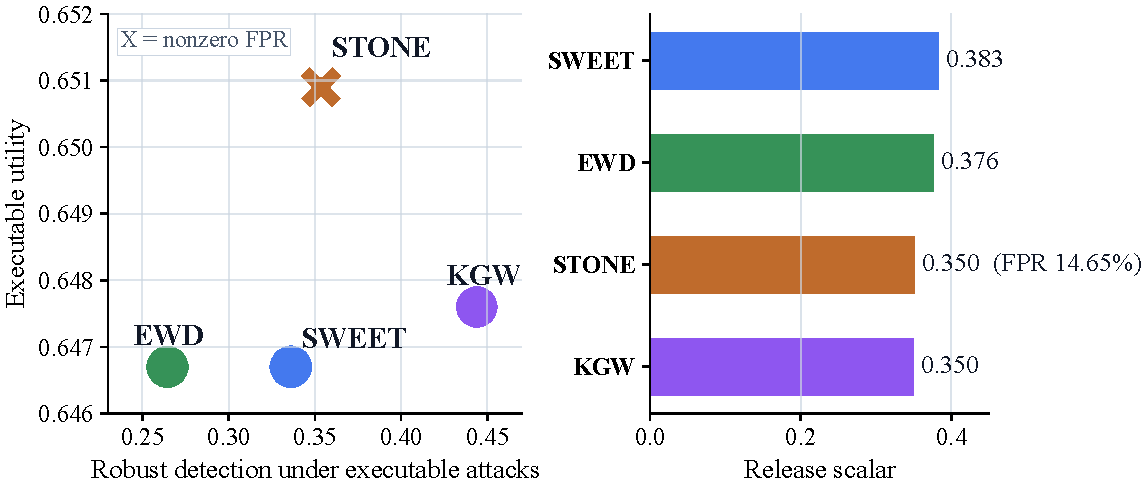
\includegraphics[width=0.96\textwidth]{fig/codemarkbench_tradeoff.pdf}
  \caption{CodeMarkBench robustness--utility tradeoff with descriptive release-scalar context. Conclusions use component coordinates and raw FPR, not a winner-takes-all ranking.}
  \label{fig:codemarkbench-tradeoff}
\end{figure}

\section{Interpretation}

The benchmark result should be read carefully. It does not imply that source-code watermarking is futile. It shows that under an executable release contract, existing runtime baselines exhibit tradeoffs across detection, robustness, utility, stealth, efficiency, and false positives. This finding motivates the rest of the dissertation. SemCodebook asks whether structured program carriers can provide stronger white-box provenance. CodeDye, ProbeTrace, and SealAudit ask how watermark evidence should be handled in black-box audit, source attribution, and safety triage settings.

More concretely, the benchmark exposes four downstream needs. Robustness and utility tradeoffs motivate SemCodebook's structured carrier design. Negative-control discipline motivates CodeDye's refusal to turn sparse black-box evidence into a prevalence claim. The fact that benchmark detection is not the same as source ownership motivates ProbeTrace's active registry. Finally, executable benchmarks still do not answer whether watermark mechanisms can interact with unsafe code behavior, which motivates SealAudit. CodeMarkBench is therefore not just an opening experiment; it supplies the problem decomposition used by the rest of the thesis.

The benchmark also clarifies how to read zero-valued cells. Zero observed negative-control hits are useful evidence only with their denominator and interval; they do not mean that a method can never fire on clean code. Conversely, a nonzero false-positive rate is not an implementation footnote. It changes the strongest claim a downstream audit can make. Additional baselines would improve benchmark breadth, but the central limitation would remain: a runtime detector observes an output-level signal, not a recoverable provenance object.

The benchmark stage therefore hands two requirements to the next stage. First, a watermark method for code should exploit program structure when such structure is available, because ordinary code edits can destroy surface evidence while preserving semantics. Second, any stronger method must inherit the benchmark's conservative accounting: parser failures, helper failures, negative controls, and recovery abstentions are evidence about the method, not rows to remove. CodeMarkBench deliberately stops before claiming a new watermarking method; it supplies the empirical reason to build one. Chapter~\ref{cpt:evidence-framework} uses this lesson to define claim-bearing rows, structured carrier recovery, and black-box audit records under one evidence model.

The practical implication is that the benchmark is not a detachable prelude. It determines how later improvements are allowed to be evaluated: recovery must preserve executable validity, sparse black-box signals must not become prevalence claims, and strong-looking attribution or triage cells must keep their source-bound or marker-hidden denominators visible. This is how the dissertation turns a benchmark release into a methodological constraint on the four later protocols.

\chapter{Watermark Evidence Framework}\label{cpt:evidence-framework}

This chapter instantiates the evidence contract from Eq.~\ref{eq:lifecycle-stage} for the first access-model break in the lifecycle. It first asks what can be recovered under the strongest evaluated access model: admitted local white-box code models with inspectable program carriers. It then asks what evidence remains when that access disappears behind a provider API. The contrast is central to the thesis: a strong white-box provenance mechanism and a sparse black-box audit signal should not be forced into the same claim type. Both stages use fixed denominators, negative controls, and explicit forbidden interpretations.

\section{Shared Evidence Model}

All modules in the dissertation distinguish claim-bearing rows from support-only rows. A claim-bearing row is a record whose task identifier, model or provider, prompt hash, output hash, detector version, threshold version, control status, decision rule, and score field are fixed before it enters the main denominator. The observed decision value is evaluated only after admission. Support-only rows may be useful for debugging, canary checks, stress exploration, or appendix examples, but they are not allowed to change the numerator or denominator of the main result.

The shared record abstraction is
\begin{equation}
  r_i=(u_i,a_i,h^p_i,h^{raw}_i,h^{struct}_i,v_D,v_\tau,c_i,d_i,s_i,b_i),
  \label{eq:claim-row}
\end{equation}
where $u_i$ identifies the task or case, $a_i$ identifies the access context such as model, provider, owner, or source group, $h^p_i$, $h^{raw}_i$, and $h^{struct}_i$ are prompt, raw-payload, and structured-payload hashes when applicable, $v_D$ and $v_\tau$ are detector and threshold versions, $c_i$ is the control or attack condition, $d_i$ is the decision, $s_i$ is the score or support statistic, and $b_i\in\{0,1\}$ marks whether the row is claim-bearing for its own lifecycle stage. Fields that are not meaningful for a specific module are stored as $\bot$ rather than removed, so every row still has a fixed schema.

Rows can be excluded before interpretation, but a diagnostic row cannot be promoted after its outcome is known. More explicitly, each module defines an admission predicate $\mathrm{Adm}_j(a_i,v_D,v_\tau,u_i,c_i)$ that depends on pre-outcome metadata such as model or provider context, detector version, threshold version, task identity, and control family. The claim-bearing flag is fixed by this predicate:
\begin{equation}
  b_i^{(j)} := \mathbf{1}[\mathrm{Adm}_j(a_i,v_D,v_\tau,u_i,c_i)=1].
\end{equation}
The main denominator is therefore
\begin{equation}
  \mathcal{D}_{main}^{(j)}=\{r_i:b_i^{(j)}=1,\ \mathrm{stage}(r_i)=j\}.
\end{equation}
The predicate is not allowed to depend on the observed decision $d_i$ or score $s_i$. This is the formal protection against outcome-dependent pruning; the flag records a pre-outcome admission decision rather than a label assigned after seeing results.

\begin{figure}[htbp]
  \centering
  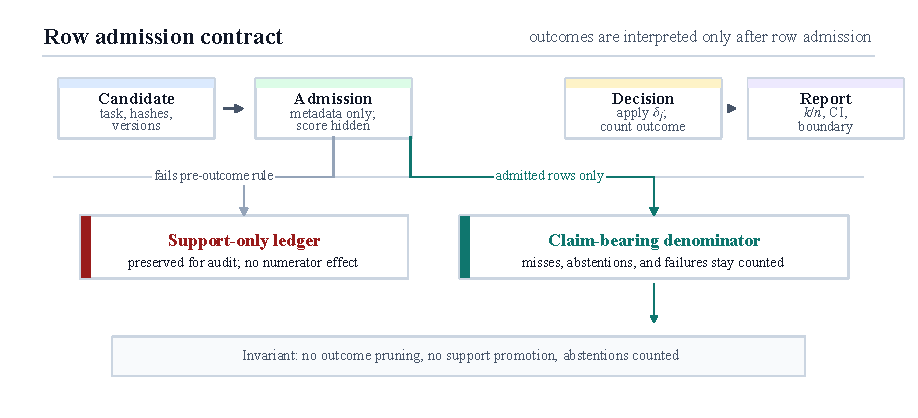
\includegraphics[width=0.96\textwidth]{fig/evidence_contract_stack.pdf}
  \caption{The row-admission contract used throughout WatermarkScope. Claim-bearing rows pass pre-outcome admission; diagnostic rows remain preserved but non-promoting.}
  \label{fig:evidence-contract-stack}
\end{figure}

\begin{algorithm}[htbp]
\caption{Evidence Admission and Claim Boundary Protocol}
\label{alg:evidence-admission}
\begin{algorithmic}[1]
\Require Candidate row $r_i$, stage $j$, frozen admission rule $\mathrm{Adm}_j$, frozen decision rule $\delta_j$
\State Bind task/case id, access context, hashes, versions, control role, and artifact path
\If{$r_i$ fails pre-outcome admission under $\mathrm{Adm}_j$}
  \State Mark $r_i$ support-only with an exclusion reason; \Return non-claim evidence
\EndIf
\State Set $b_i\gets 1$ and lock $r_i$ into denominator $\mathcal{D}^{(j)}_{\mathrm{main}}$
\State Evaluate $d_i \gets \delta_j(r_i)$
\If{$d_i$ is abstain, reject, miss, no-signal, or needs-review}
  \State Record the non-success outcome; the row remains inside $\mathcal{D}^{(j)}_{\mathrm{main}}$
\EndIf
\State Add to the numerator only when $d_i$ matches the predeclared event
\State Report $k/n$, uncertainty, support-only exclusions, and forbidden interpretations
\end{algorithmic}
\end{algorithm}

Algorithm~\ref{alg:evidence-admission} does not prove that a detector is correct. It defines when a row may support a claim and when it must remain support-only. This is why the dissertation can report strong SemCodebook recovery, sparse CodeDye signals, perfect scoped ProbeTrace attributions, and high-abstention SealAudit triage without collapsing them into one misleading score.

For example, a canary row with complete hashes can still be support-only if it was generated for a diagnostic prompt outside the frozen live denominator. Excluding that row is not cherry-picking when the exclusion was determined before seeing its decision. It would become cherry-picking only if the row were promoted because it made the numerator look better. This distinction is important for CodeDye and SealAudit, where support rows remain valuable for auditability but cannot change the main result.

For a result with $k$ observed events over $n$ claim-bearing records, the observed rate is
\begin{equation}
  \hat{p} = \frac{k}{n}.
\end{equation}
When reporting uncertainty, the dissertation uses Wilson-style confidence intervals~\cite{wilson1927probable}; the formula and zero-event convention are given in Appendix~\ref{app:artifact-index}, Table~\ref{tab:stat-reporting-rules}. These intervals are row-level descriptive intervals over admitted rows, not cluster-adjusted generalization intervals across future models, providers, owners, or tasks; clustered support surfaces are separately marked by task, model family, language, or attack family.

\section{SemCodebook: White-Box Provenance}

SemCodebook is the response to the benchmark's robustness--utility lesson: it changes the evidence object from a surface detector score to a recoverable structured identifier. It is designed for admitted white-box family and scale cells. Its goal is not merely to detect that some signal exists, but to recover a structured provenance identifier under semantic-preserving transformations. The implementation uses named rewrite/carrier families whose metadata are backed by AST-, CFG-, and SSA-style evidence. The report groups those implementation families by structural level:
\begin{equation}
  C(x) =
  \bigsqcup_{r\in\{\mathrm{AST},\mathrm{CFG},\mathrm{SSA}\}}
  \{(r,z): z\in C_r(x)\},
  \label{eq:carrier-extraction}
\end{equation}
where $\bigsqcup$ denotes a tagged disjoint union over structural evidence levels rather than a claim that the code contains only three literal carrier types. This notation is important because an AST-backed rewrite, a CFG-backed rewrite, and an SSA-style data-flow rewrite are not interchangeable even if their textual realization overlaps.
The carrier families play different roles. AST-backed carriers capture syntactic structure that survives many formatting and naming changes. CFG-backed carriers capture execution-order structure and therefore help when local syntax is rewritten but control dependencies remain recognizable. SSA-style carriers capture data-flow support, which is useful when expression-level changes preserve value dependencies. The method does not assume that every carrier family is available in every artifact; it assumes that carrier availability is measured and that insufficient support causes abstention instead of silent fallback.

A useful way to read SemCodebook is as a recovery protocol rather than as a decorative marker. The embedder chooses where the evidence may live, the executable harness checks whether the modified program remains valid, and the detector attempts to recover a provenance identifier under the same typed schedule. A row can therefore fail by missed recovery, support-gate rejection, carrier insufficiency, helper/compiler failure, or negative-control firing. All of these outcomes are more informative than a detector-only pass/fail result. The implementation schedule is adaptive: carrier families are first scored for applicability, then ranked by a frozen mixture of applicability, family prior, and keyed tie-breaking. A compact mathematical abstraction of that implementation is
\begin{align}
  q_f(x,K) &= \alpha\,a_f(x)+\beta\,b_f+\gamma\,u_f(K),\\
  \sigma_K(x) &= \mathrm{TopSlots}\bigl(\mathrm{sort}_{q_f}(F_x)\bigr),
  \label{eq:keyed-schedule}
\end{align}
where $F_x$ is the set of implementation carrier families considered for artifact $x$, $a_f(x)$ is measured applicability, $b_f$ is a frozen family bias, and $u_f(K)$ is the HMAC-derived tie-break value for the carrier key. The submitted implementation uses the resulting schedule to choose data slots and an anchor slot; Eq.~\eqref{eq:keyed-schedule} is therefore a faithful abstraction of the code path, not a second independent algorithm.
If no carrier family is applicable, or the family coverage is below the recovery threshold after row admission, the detector abstains and the outcome remains inside the positive denominator. By contrast, pre-run failures such as an unavailable model revision, missing parser, or missing helper/dependency closure produce a nonpromotion audit before the row enters the denominator. Encoded bit positions are assigned to scheduled implementation families; if the selected family has no admissible carrier, the row abstains instead of being silently moved to another family.
The carrier schedule is fixed before the checksum is formed:
\begin{equation}
  \kappa = H(\mathrm{payload}\Vert \sigma_K(x)\Vert v_{\mathrm{sched}}).
\end{equation}
The public schedule digest record is
\begin{equation}
  \mathrm{schedule\_digest}=H(K_{\mathrm{pub}}\Vert t\Vert \sigma_K(x)\Vert \kappa).
\end{equation}
Here $v_{\mathrm{sched}}$ is the frozen schedule/recovery protocol version, and $K_{\mathrm{pub}}$ is a public digest salt or verification key rather than the embedding secret $K$; the dissertation uses the digest for version binding and traceability, not as a cryptographic hiding commitment.
The watermark payload is then decoded through an ECC-style schedule block:
\begin{equation}
  \mathbf{c} = \mathrm{ECC\_Encode}(\mathrm{payload}).
\end{equation}
The schedule digest and positive-support certificate are recorded as row-level validation evidence. ECC failure, decoded-payload mismatch, incomplete positive-support evidence, and schedule-support insufficiency are counted as reject, abstain, or miss outcomes in the positive denominator, not removed from the result.
At detection time, each scheduled carrier yields a soft observation $o_i \in \{0,1,\mathrm{erasure}\}$, and the recovered payload candidate is
\begin{equation}
  \widehat{\mathrm{payload}} = \mathrm{ECC\_Decode}(o_1,\ldots,o_L).
\end{equation}
Recovery is accepted only when the decoded payload matches the expected identifier and the positive-support and schedule-commitment evidence are valid under the frozen detector version. A decoded candidate without that supporting evidence is counted as a reject, abstain, or miss, not as a recovery.

The full embed and recover pseudocode is moved to Appendix~\ref{app:reproducibility} so that the main body can keep the lifecycle argument visible. Operationally, SemCodebook has four phases: extract typed carrier evidence, schedule implementation families with a frozen key, materialize only executable-preserving carriers, and recover an identifier only when ECC-style decoding, payload matching, schedule commitment, and positive-support evidence agree. Failed materialization, insufficient carriers, ECC rejection, decoded-payload mismatch, and support-gate failure remain inside the appropriate admitted denominator rather than being removed after the fact.

The current SemCodebook evidence surface contains 72,000 structured white-box records across 10 admitted models and 5 model families. The positive detector surface contains 23,342 recoveries over 24,000 claim-bearing positives, or 97.26\%. The negative-control surface contains 0 hits over 48,000 controls. The current ablation surface contains 43,200 generation-changing rows. Table~\ref{tab:semcodebook-results} summarizes the claim-safe result.

This is the largest positive recovery surface in the dissertation under the strongest evaluated access model: local white-box code models with typed carrier inspection and executable admission. The pooled rate is used as the main-body headline only. The claim-bearing artifact records per-model, per-family, per-language, and per-attack intervals separately, and those cell-level summaries are required for any final paper table. This prevents a large or easy cell from silently dominating the interpretation.

An admitted SemCodebook cell must satisfy four pre-run conditions: the model is a local white-box code model with a frozen revision, the source group has executable tests, the language parser and carrier extractor are available, and the helper/dependency closure can be validated. The full gate table is in Appendix~\ref{app:reproducibility}, Table~\ref{tab:sem-admission-app}. A failed parser, missing helper closure, or unavailable model revision produces a nonpromotion audit rather than a smaller denominator.

\begin{table}[htbp]
\centering
\caption{SemCodebook claim-bearing denominators and control surface. Structured-row and ablation-row counts are coverage/support evidence and do not alter the recovery denominator.}
\label{tab:semcodebook-results}
\compacttable
\begin{tabularx}{\textwidth}{@{}L{2.85cm}L{2.25cm}Y@{}}
\toprule
Quantity & Value & Interpretation \\
\midrule
Recoveries & 23,342/24,000 & 97.26\%; 95\% CI about 97.04--97.46\% \\
Miss/abstain/reject & 658/24,000 & Included in positive denominator \\
Neg. control hits & 0/48,000 & 0 observed; 95\% upper bound about 0.008\% \\
Coverage/support & 72,000; 43,200 & Structured records and ablation rows; support evidence only \\
\bottomrule
\end{tabularx}
\end{table}

\begin{figure}[htbp]
  \centering
  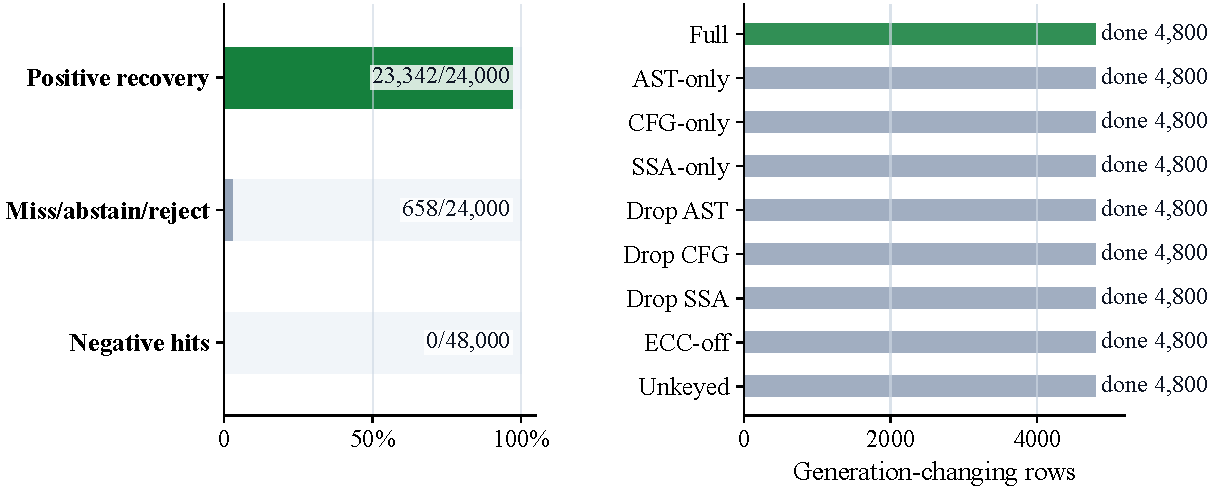
\includegraphics[width=0.96\textwidth]{fig/semcodebook_ablation.pdf}
  \caption{SemCodebook claim surface and ablation coverage. The figure separates main claim evidence from support-only ablation coverage, preserving the denominator boundary used throughout WatermarkScope.}
  \label{fig:semcodebook-ablation}
\end{figure}

The allowed SemCodebook claim is therefore rate-bound and scoped: it achieves the reported recovery and control rates within admitted white-box family and scale cells. The result also explains why the next stage is necessary. This is the first major access-model break in the dissertation. Once the model is accessed only through a provider API, the auditor can no longer inspect carrier families, helper closure, or ECC recovery state. The evidence object must change from a recoverable structural identifier to a preserved black-box transcript. This access-model break is the reason CodeDye is framed as null-audit rather than as a weaker version of SemCodebook.

The ablation design is important for scientific interpretation. The dissertation uses the promoted 43,200-row ablation gate as evidence that the major component interventions were executed under a fixed design: full AST/CFG/SSA/ECC/keyed scheduling, three single-family arms, three drop-family arms, ECC-off, and unkeyed scheduling. The ablation is reported as a promotion gate because the compact artifact binds arm counts and hash evidence; full per-arm rates remain artifact-level evidence. This keeps the main body honest: it shows that the causal questions were instrumented without inventing unsupported effect sizes in the report.

\section{CodeDye: Conservative Black-Box Null-Audit}

When carrier access disappears behind a provider API, the evidence object changes from recovery to transcript preservation. CodeDye implements this black-box audit stage. In this setting, the auditor cannot inspect model weights, carriers, helper closure, or training data. The protocol therefore records evidence rather than forcing a strong contamination claim. The implementation distinguishes a statistics-artifact signal definition from the final reporting signal: the statistics artifact records 4/300 rows under one narrow definition, while the final frozen reporting surface records 6/300 sparse audit signals. They are reported separately and are not combined. A CodeDye audit record is the black-box projection of Eq.~\ref{eq:claim-row}:
\begin{equation}
  \tilde{r}_i = (t_i, h^{p}_i, h^{raw}_i, h^{struct}_i, \mathbf{g}_i, v_D, v_{\tau}),
\end{equation}
where $\tilde{r}_i$ is the black-box projection of the full row schema: omitted fields are inherited as $c_i$, $d_i=\mathrm{signal}^{report}_i$, $s_i$ records the staged evidence summary, and $b_i=1$ only for admitted live rows. Here $h^{p}_i$ is the prompt hash, $h^{raw}_i$ is the raw response hash, $h^{struct}_i$ is the structured payload hash, $\mathbf{g}_i$ is the frozen detector gate vector, and $v_D$ and $v_{\tau}$ identify detector and threshold versions. Earlier design notes used a schematic linear score, but the claim-bearing frozen protocol uses a non-weighted familywise gate. This avoids hiding a failed evidence channel behind a high score from another channel. Let
\begin{equation}
  \mathbf{g}_i=(g^{fam}_i,g^{struct}_i,g^{direct}_i,g^{weak}_i,g^{ctx}_i)\in\{0,1\}^5
\end{equation}
record family observation, structural or stable witness evidence, direct canary evidence, weak canary evidence, and heldout/rewrite context evidence. Hash retention and chronology fields are admission/audit metadata for the row; the detector-stage reporting event is the implementation evidence stage:
\begin{align}
  \mathrm{signal}^{report}_i
  = \mathbf{1}\bigl[\mathrm{stage}(\mathbf{g}_i,\mathrm{witness}_i,\mathrm{density}_i)=4\bigr].
\end{align}
All thresholds and predicate components are fixed by the detector and threshold versions before a claim-bearing run.
The narrower statistics-artifact predicate is denoted $\mathrm{signal}^{stats}_i$ and is stored under a different threshold version:
\begin{equation}
  \mathrm{signal}^{stats}_i =
  \mathbf{1}[s^{stats}_i \geq \tau_{stats} \wedge \mathrm{hashes\_valid}_i].
\end{equation}
The numerator event uses $\mathrm{signal}^{report}_i$ only, and the denominator remains the admitted 300 live rows. The two predicates are not added together.

Appendix~\ref{app:reproducibility}, Table~\ref{tab:protocol-sketches}, gives the frozen null-audit decision sketch. In the main text, the important point is the non-weighted gate: family evidence, structural or stable witness evidence, canary evidence, and context evidence must support the final evidence stage before a row is reported as a sparse signal. A failure after row admission remains a no-signal or failure inside the 300-row denominator.

The current DeepSeek live claim surface contains 300 rows. CodeDye observes 6 sparse audit signals over those 300 rows, or 2.00\%. Positive contamination controls fire in 170/300 cases, while negative controls show 0/300 hits. In addition, 806 support rows are explicitly excluded from the main denominator. Table~\ref{tab:codedye-results} summarizes the result.

\begin{table}[htbp]
\centering
\caption{CodeDye live audit, controls, and support-row exclusions. The live signal is sparse audit yield, not prevalence.}
\label{tab:codedye-results}
\compacttable
\begin{tabularx}{\textwidth}{@{}L{2.45cm}L{2.00cm}Y@{}}
\toprule
Quantity & Value & Interpretation \\
\midrule
Live rows & 300 & Main claim denominator \\
Sparse live signals & 6/300 & 2.00\%; 95\% CI about 0.92--4.29\% \\
Positive controls & 170/300 & 56.67\%; 95\% CI about 51.0--62.2\% \\
Neg. control hits & 0/300 & 0 observed; 95\% upper bound about 1.26\% \\
Excluded support rows & 806 excluded & Retained for auditability; all excluded from the live denominator before interpretation \\
\bottomrule
\end{tabularx}
\end{table}

The intervals in Table~\ref{tab:codedye-results} are row-level Wilson intervals over admitted rows. They are not provider-general guarantees, and zero observed negative hits should be read with the printed upper bound rather than as zero false-positive risk.

The correct interpretation is a curator-side null-audit. The result is intentionally not written as contamination prevalence, provider accusation, or high-recall detection. A sparse live signal means that the frozen non-weighted evidence stage fired under the submitted audit predicate, but a no-signal row is not proof that the provider never saw related material. The value of the protocol is that it preserves evidence and prevents a weak black-box signal from being inflated into a stronger claim.

This conservative treatment is essential for academic integrity. A black-box provider response can be affected by prompt wording, retrieval-like behavior, decoding variation, and hidden moderation or safety layers. CodeDye therefore treats positive controls and negative controls as calibration evidence, while the live 6/300 signal is reported only as sparse audit yield.

This leaves one final gap. A preserved transcript can support an audit trail, but it still does not identify which registered source or owner can claim the evidence, and it does not say whether acting on the evidence is safe. Chapter~\ref{cpt:attribution-triage} therefore adds two governance layers rather than another detector: ProbeTrace binds evidence to a pre-registered owner under false-owner controls, and SealAudit routes marker-hidden risk without unsafe pass-through. Both stages keep the same denominator discipline introduced here.

This handoff defines the chapter's role in the lifecycle. SemCodebook shows what is possible when the defender can use program structure and local model access; CodeDye shows what remains defensible after those assumptions disappear. The shared contribution is not that both stages optimize the same metric. It is that both stages use the same evidence rule: the row is admitted before the result is known, controls are reported with the result, and the strongest claim is limited by the available evidence object. The next chapter applies that rule to two questions that arise only after evidence exists: who can claim it, and whether it should trigger security review.

This distinction is the main methodological bridge from watermarking to governance. A recoverable identifier answers a provenance question, while a preserved transcript answers an audit question. Neither, by itself, decides ownership or safety. The next stage therefore does not try to inflate CodeDye's sparse signal or reinterpret SemCodebook's white-box recovery as black-box detection. It adds the missing assumptions explicitly: an owner registry for attribution and a marker-hidden evidence vector for triage.

\chapter{Attribution and Security Triage}\label{cpt:attribution-triage}

After CodeDye preserves black-box evidence, the lifecycle reaches two deployment questions that transcript evidence alone cannot answer: who can make a scoped source claim, and whether acting on the evidence is safe. ProbeTrace adds the missing owner-registry assumption for active-owner attribution; SealAudit then treats the watermarking mechanism itself as a security-relevant object. This chapter is therefore the deployment end of WatermarkScope, not a pair of unrelated follow-up projects.

\section{ProbeTrace: Active-Owner Source-Bound Attribution}

ProbeTrace is not a universal authorship detector. It is an active-owner attribution protocol. The owner registry is written as
\begin{equation}
  \mathcal{R} = \{(o, K_o, h^{split}_o): o\in O\},
\end{equation}
where $K_o$ is the owner key and $h^{split}_o$ identifies the source split or registry commitment associated with that owner. For an output $x$, ProbeTrace computes an owner-specific witness score
\begin{equation}
  s_o(x)=\mathrm{witness\_score}(x,K_o,h^{split}_o).
\end{equation}
The score is normalized to $[0,1]$, with larger values indicating stronger agreement with the registered owner witness. The current claim surface is single-active-owner and source-bound. Let $\mathcal{C}_{wrong}(x)$, $\mathcal{C}_{null}(x)$, and $\mathcal{C}_{rand}(x)$ denote the wrong-owner, null-owner, and random-owner control evidence attached to the same APIS claim surface. The operational scenario is deliberately narrow: before evaluation, the owner registry and source-split commitment are fixed; during evaluation, the active owner must pass its frozen witness threshold while the available control evidence remains below its frozen acceptance boundary. The full decision function is $\delta_{PT}(x)\in\{\mathrm{attribute},\mathrm{reject},\mathrm{abstain}\}$; the following indicator is the protocol contract for the success event:
\begin{align}
  \mathrm{attr}_o(x)
  = \mathbf{1}\bigl[
  &s_o(x)\geq\tau_o
  \wedge \max_{c\in\mathcal{C}_{wrong}(x)}c<\tau_{wrong} \nonumber\\
  &\wedge\ \max_{c\in\mathcal{C}_{null}(x)}c<\tau_{null}
  \wedge \max_{c\in\mathcal{C}_{rand}(x)}c<\tau_{rand}
  \bigr].
\end{align}
A row is admitted to this APIS decision only when the active evidence, owner-control evidence, and their threshold or artifact versions are present in the preserved claim surface. If a required control family is missing before evaluation, the row is nonpromoted; if evidence becomes insufficient after admission, the decision rule returns reject or abstain inside the APIS denominator.
A future multi-owner protocol over a simultaneous registry $\mathcal{R}_{multi}$ would additionally use the margin
\begin{align}
  o^\ast &= \arg\max_o s_o(x),\\
  \Delta(x) &= s_{o^\ast}(x)-s_{\mathrm{second}}(x).
\end{align}
Here $s_{\mathrm{second}}(x)$ is the second-largest score over a simultaneous registry. Because explicit comparable margin fields are not available for every APIS row, this margin expression is presented as protocol design rather than as a validated APIS-300 margin claim. If the active score is below the evidence threshold, the current protocol abstains for insufficient evidence. If a future multi-owner margin is below $\tau_{\Delta}$, the multi-owner protocol abstains for ambiguity.

The compact decision sketch is included in Appendix~\ref{app:reproducibility}, Table~\ref{tab:protocol-sketches}. The main-body claim is that a row succeeds only when the active owner passes and all same-task owner controls stay below their frozen thresholds. If either side of that conjunction fails, the protocol rejects or abstains inside the APIS denominator. This is closer to a controlled audit protocol than to open-world authorship attribution.

The current ProbeTrace claim-bearing surface contains 300 APIS attribution records in the scoped active-owner setting and 1,200 false-owner controls. It observes 300/300 APIS success events under the scoped APIS protocol and 0/1,200 false-owner hits. Separately, 900 source-bound transfer rows are support-only receipt/source-binding evidence over 300 task clusters. Within the APIS-300 denominator, no insufficient-evidence abstention is counted as a success; an abstention would have entered the denominator as a non-attribution outcome. The transfer rows are reported with task-cluster sensitivity: the primary independence unit is the task identifier rather than treating all 900 rows as fully independent tasks. Table~\ref{tab:probetrace-results} summarizes the result.

\begin{table}[htbp]
\centering
\caption{ProbeTrace attribution-stage evidence surface. The allowed claim is source-bound, single-active-owner attribution under the evaluated protocol only.}
\label{tab:probetrace-results}
\compacttable
\begin{tabularx}{\textwidth}{@{}L{2.45cm}L{2.00cm}Y@{}}
\toprule
Quantity & Value & Interpretation \\
\midrule
Scoped APIS decisions & 300/300 attributed & APIS success events under frozen single-owner protocol; Wilson 95\% lower bound about 98.74\% \\
False-owner controls & 0/1,200 & 0 observed; 95\% upper bound about 0.32\% \\
\addlinespace[2pt]
\multicolumn{3}{@{}l}{\emph{Support-only evidence}}\\
Transfer support rows & 900 support-only & Receipt-complete source-binding support over 300 task clusters; not part of the APIS attribution denominator \\
\bottomrule
\end{tabularx}
\end{table}

The three ProbeTrace evidence surfaces have different meanings. APIS-300 measures attribution under the frozen active-owner protocol. The 1,200 controls measure whether wrong, null, or random owner evidence falsely passes. The 900 transfer rows are support-only: they check receipt completeness and source binding under student-transfer variants, with 300 task clusters as the primary independence unit, but they do not enlarge the main attribution denominator. This separation matters because a single large number would make the result look stronger but less honest. The intervals reported for ProbeTrace are row-level Wilson intervals over admitted rows and are conditional on this scoped protocol.

The result is strong for the scoped setting, but the perfect observed rate requires careful writing. The dissertation does not claim multi-owner generalization, provider-general attribution, broad authorship detection, or validated margin separability. The current result also has practical caveats: some positives are near-boundary or low-confidence under diagnostic margin analysis, and the protocol has nontrivial query and latency cost. The claim is that active-owner and source-bound evidence can be useful under the evaluated protocol and controls, not that every attribution instance is equally strong.

The main examiner risk is that 300/300 appears too perfect. The dissertation handles this by reporting false-owner controls, transfer receipt integrity, and task-cluster sensitivity. In other words, the result is presented as a scoped protocol success rather than a universal attribution theorem. If future work adds multi-owner experiments, those experiments should introduce wrong-owner, null-owner, random-owner, and owner-heldout controls before any broader claim is made.

\section{SealAudit: Watermark-as-Security-Object Triage}

Attribution does not certify safety. Even if ProbeTrace binds an output to a registered source, that evidence does not say whether the watermarking or marker mechanism changes security-relevant behavior. SealAudit therefore changes the question from source binding to risk triage. The evidence object is no longer an owner witness; it is a marker-hidden audit row that can be benign, latent risk, or retained for review. This is the final handoff in the lifecycle: after a system can evaluate, recover, audit, and attribute evidence, it still needs to decide whether the evidence mechanism itself is safe enough to act on.

SealAudit treats watermark markers and related mechanisms as security-relevant objects. The key design choice is selective triage. For each row, the resolver receives an evidence vector
\begin{equation}
  e_i=(e^{static}_i,e^{semantic}_i,e^{launder}_i,e^{spoof}_i,e^{judge}_i),
\end{equation}
covering static safety, semantic drift, laundering, spoofability, and provider-judge perturbation evidence when available. The conservative resolver is described as a function $g(e_i)\rightarrow \mathcal{Y}$ that returns a decisive label only when component evidence is sufficient and non-conflicting. In the submitted artifacts, these semantics are stored as row-level final decisions and unsafe-pass flags rather than recomputed from raw component scores during the PDF build. The normalized decision set is
\begin{equation}
  \mathcal{Y} = \{\mathrm{benign}, \mathrm{latent\_risk}, \mathrm{needs\_review}\}.
\end{equation}
The artifact labels \emph{confirmed\_benign} and \emph{confirmed\_latent\_risk} are mapped to the normalized decisive labels \emph{benign} and \emph{latent\_risk} in the report. Let $S(e_i)$ denote sufficient evidence for a decisive label and $Q(e_i)$ denote a conflict among evidence components. These are the adjudication semantics used to interpret the stored row decisions; they do not depend on the final table counts. The resolver contract is conservative:
\begin{equation}
  g(e_i)=\mathrm{needs\_review}
  \quad\text{if}\quad
  \neg S(e_i)\ \vee\ Q(e_i).
\end{equation}
When $S(e_i)\wedge\neg Q(e_i)$ holds, a frozen subrule $h(e_i)$ selects the decisive output:
\begin{equation}
  g(e_i)=h(e_i)\in\{\mathrm{benign},\mathrm{latent\_risk}\}.
\end{equation}
For example, a marker-hidden case with clean static evidence but unstable semantic behavior under laundering should not be forced into benign. It is routed to needs-review because the evidence components disagree. A decisive benign row requires enough non-conflicting evidence to make the risk interpretation stable under the evaluated checks.
Coverage and safety are reported separately over the marker-hidden row denominator $n=960$. Let $y_i^\ast$ be the adjudicated or construction-derived reference state for row $i$, and let $\hat{y}_i$ be the triage output. In $y_i^\ast$, \emph{needs\_review} denotes a should-review reference state caused by unresolved or conflicting evidence; it is not treated as a hidden ground-truth class equivalent to benign or latent risk. The unsafe-pass count is not a returned class; it is an audit error event in which evidence that should require risk or review is incorrectly allowed through as benign:
\begin{equation}
  \mathcal{Y}^{\ast}_{block}=\{\mathrm{latent\_risk},\mathrm{needs\_review}\}.
\end{equation}
\begin{align}
  \mathrm{Coverage} &= \frac{1}{n}\sum_i \mathbf{1}[\hat{y}_i\in\{\mathrm{benign},\mathrm{latent\_risk}\}],\\
  \mathrm{NeedsReviewRate} &= \frac{1}{n}\sum_i \mathbf{1}[\hat{y}_i=\mathrm{needs\_review}],\\
  \mathrm{UnsafePassRate} &=
  \frac{1}{n}\sum_i
  \mathbf{1}[y_i^\ast\in\mathcal{Y}^{\ast}_{block}
  \wedge \hat{y}_i=\mathrm{benign}].
\end{align}
This is an all-hidden-row unsafe-pass rate. A conditional unsafe-pass rate over block-required rows would require a separately fixed block denominator; the submitted surface reports the all-row audit-error event instead. This is more appropriate than accuracy or F1 when the system is designed to abstain under insufficient or conflicting evidence.

The resolver decision sketch is included in Appendix~\ref{app:reproducibility}, Table~\ref{tab:protocol-sketches}. The main-body rule is that insufficient evidence or component conflict returns needs-review before any benign or latent-risk label is allowed. The verification script checks the stored final decision, marker-hidden claim role, required evidence fields, and unsafe-pass flag; it does not silently reinterpret visible-marker diagnostics as hidden claim rows.

The current SealAudit claim surface contains 320 cases and 960 marker-hidden rows. It reports 81 decisive outcomes, 879 needs-review outcomes, and 0 unsafe-pass outcomes. Marker-visible rows are diagnostic-only and do not enter the marker-hidden claim denominator. A correct owner attribution can still point to unsafe or ambiguous code; therefore attribution is not the endpoint of the lifecycle. Table~\ref{tab:sealaudit-results} summarizes the result.

\begin{table}[htbp]
\centering
\caption{SealAudit triage-stage marker-hidden evidence surface. Marker-visible rows are diagnostic-only and are excluded from the hidden denominator.}
\label{tab:sealaudit-results}
\compacttable
\begin{tabularx}{\textwidth}{@{}L{2.45cm}L{2.00cm}Y@{}}
\toprule
Quantity & Value & Interpretation \\
\midrule
Hidden rows & 960 & Main claim denominator \\
Decisive & 81/960 & 8.44\%; 95\% CI about 6.84--10.37\%; 80 benign and 1 latent risk \\
Needs review & 879/960 & 91.56\%; 95\% CI about 89.63--93.16\% \\
Unsafe pass & 0/960 & 0 observed; 95\% upper bound about 0.40\% \\
\bottomrule
\end{tabularx}
\end{table}

The intervals in Table~\ref{tab:sealaudit-results} are row-level Wilson intervals over the submitted marker-hidden denominator. They are not deployment-wide safety guarantees; zero observed unsafe passes should be read with the printed upper bound.

SealAudit is therefore a selective risk-audit protocol, not a security certificate. Its main contribution is that it refuses to collapse ambiguous or under-supported cases into confident labels. In safety-sensitive settings, an explicit needs-review outcome is often preferable to a misleading automatic decision.

The high needs-review rate is not hidden because it is part of the safety story. An automatic classifier with higher coverage but unknown unsafe-pass behavior would be less defensible. SealAudit instead reports coverage and unsafe-pass separately, which lets a human reviewer decide whether the current frontier is useful for triage, whether more evidence is required, or whether a case should be escalated to expert review.

The practical value is therefore workload shaping rather than full automation. The 81 decisive marker-hidden outcomes identify cases that can be handled with the current evidence conjunction, while the remaining 879 cases are explicitly retained for review instead of being forced into labels. For an examiner, the key question is not whether 8.44\% coverage is high; it is whether the protocol reduces obvious review work without silently passing unsafe cases. The current evidence supports that narrower claim and leaves coverage improvement as future work.

\section{Deployment Governance Synthesis}

ProbeTrace and SealAudit close the lifecycle by separating ownership evidence from safety evidence. Attribution may be strong in one scoped setting, while security triage may still require abstention. A credible source-code watermarking framework therefore needs both: source-bound evidence for ownership questions and marker-hidden triage for risk questions.
At this point the lifecycle has evaluated benchmark evidence, embedded structured provenance, traced black-box and owner-bound evidence, and audited security-relevant marker behavior under progressively weaker or riskier access settings.

This separation is important for deployment. A system operator who receives a ProbeTrace attribution still needs to know whether the associated marker or generated artifact should be accepted, escalated, or reviewed. Conversely, a SealAudit needs-review outcome does not prove that the source claim is false; it says that the security evidence is not decisive enough for automatic action. The two modules therefore produce complementary governance outputs: one binds evidence to a scoped owner, and the other prevents that evidence from becoming an unchecked safety decision.

The chapter also explains the dissertation's conservative treatment of perfect and weak-looking results. ProbeTrace is written narrowly because perfect APIS observations would be easy to overclaim without the owner-registry boundary. SealAudit is written as selective triage because high abstention is preferable to unsafe pass-through in a security-sensitive setting. These choices are not rhetorical downgrades; they are the access-model discipline required before Chapter~\ref{cpt:discussion} compares the five evidence surfaces.

The deployment lesson is that a watermarking system should produce reviewable evidence, not only automatic labels. In a real code-generation workflow, the cost of a false ownership claim, a false contamination claim, or an unsafe benign label can be higher than the cost of abstaining. ProbeTrace and SealAudit make this explicit by separating source evidence from risk evidence. A scoped attribution can be useful without being universal, and a low-coverage triage system can be useful if it preserves an unsafe-pass boundary.

This completes the lifecycle needed for the final synthesis. CodeMarkBench evaluates the denominator, SemCodebook embeds recoverable structure, CodeDye traces black-box evidence, ProbeTrace binds source ownership under a registry, and SealAudit audits marker-hidden risk. Chapter~\ref{cpt:discussion} compares these evidence surfaces without turning them into one misleading accuracy score.

The deployment framing is therefore intentionally two-handed. ProbeTrace shows how a strong owner-bound result can be made defensible by narrowing the registry and control assumptions. SealAudit shows how a weak-looking coverage result can still be useful when the objective is to avoid unsafe automatic pass-through. Both results would be easier to advertise if their boundaries were removed, but they would become much harder to defend. The final chapter keeps the boundaries visible and treats them as part of the contribution.

This is also where the lifecycle becomes practically useful for a future deployment or paper submission. ProbeTrace says which owner-bound evidence is strong enough to support a source claim under a fixed registry. SealAudit says whether the same evidence should be acted on automatically, escalated, or retained for review. A deployment system needs both decisions because the cost of an unsupported source claim and the cost of an unsafe benign decision are different. The chapter therefore closes with a separation of duties: attribution can bind evidence to a source, but triage decides whether the evidence is safe to use. That separation is the reason the final synthesis compares result surfaces by access contract rather than by one shared accuracy score.

For the FYP implementation, this separation is reflected in the artifacts. ProbeTrace rows bind an active witness, owner-control evidence, and transfer-support manifests. SealAudit rows bind marker-hidden decisions, visible-marker diagnostics, and unsafe-pass events. The two modules are stored together in the lifecycle because both are deployment-facing, but their denominators are intentionally not merged. A merged denominator would make the project look tidier while destroying the meaning of both results: attribution rows do not measure safety, and triage rows do not measure source ownership.

This is the main design lesson before the synthesis chapter. Watermark evidence becomes more useful as it moves toward deployment only when the system also becomes more explicit about what it refuses to decide. ProbeTrace refuses open-world authorship, and SealAudit refuses automatic classification under ambiguity. The next chapter uses that refusal as a positive criterion for comparing the five stages.

The practical effect is that WatermarkScope separates two decisions that are often conflated in provenance discussions. The first decision is evidential: whether a row supports a bounded source or audit claim under a fixed registry, transcript, or marker-hidden record. The second decision is operational: whether the evidence should be accepted automatically, escalated, or retained for review. ProbeTrace mainly answers the first question; SealAudit mainly answers the second. This separation makes the deployment story more cautious, but it also makes it harder for a reviewer to attack the work as a detector pretending to be an end-to-end governance system.

\chapter{Evaluation Synthesis and Discussion}\label{cpt:discussion}

The dissertation is best read as one research line rather than five independent demonstrations. CodeMarkBench defines an executable denominator; SemCodebook turns the benchmark lesson into structured white-box provenance; CodeDye shows what remains auditable when model internals disappear; ProbeTrace adds an owner registry for source-bound attribution; and SealAudit asks whether watermark evidence should trigger security review. This chapter compares those stages without forcing them into one weighted score.

\section{Synthesis Protocol}

The synthesis uses three rules. First, a result is interpreted through the evidence object it actually measures. A 97.26\% SemCodebook recovery rate and a 2.00\% CodeDye sparse-signal rate are not competing accuracies: one is a white-box provenance recovery event, and the other is a black-box null-audit event. Second, strong-looking numbers are paired with controls or abstentions. ProbeTrace's 300/300 APIS result is read with false-owner controls and single-owner scope; SealAudit's 0 unsafe-pass observation is read with high needs-review coverage. Third, support-only evidence remains non-promoting. Ablations, transfer rows, visible-marker diagnostics, and continuation plans may motivate later work, but they do not alter a submitted denominator.

These rules fit source-code watermarking because a generated program is not merely a string, and a detector output is not automatically provenance, ownership, contamination evidence, or safety evidence. Each transition in WatermarkScope changes either access or risk: executable benchmark rows become inspectable carriers, carriers become preserved transcripts, transcripts become owner-bound witnesses, and owner-bound evidence becomes marker-hidden triage. The useful question is therefore whether each stage reports the strongest claim supported by its access model.

\section{Cross-Stage Result Surface}

Table~\ref{tab:main-results} is the compressed result surface of the dissertation. It is not a leaderboard. The columns identify the counted object, the observed outcome, and the strongest reading that survives the controls.

\begin{table}[htbp]
\centering
\caption{Main quantitative result surfaces. Denominators are fixed within modules and are not interchangeable across modules.}
\label{tab:main-results}
\tighttable
\begin{tabularx}{\textwidth}{@{}L{1.72cm}L{2.35cm}L{2.95cm}Y@{}}
\toprule
Lifecycle stage & Main denominator & Observation & Safe reading \\
\midrule
Benchmark & 140 model-method-source runs & 140/140 complete; no method dominates all dimensions. & Finite executable release matrix. \\
Provenance & 24,000 positives; 48,000 negatives & 23,342 recovered; 0 negative hits. & Admitted-cell white-box provenance evidence. \\
Audit & 300 live rows plus fixed controls & 6 sparse live signals; 170/300 positive controls; 0/300 negative controls. & Null audit, not prevalence. \\
Attribution & 300 APIS rows; 1,200 false-owner controls & 300 scoped attributions; 0 false-owner hits. & Single active owner only. \\
Triage & 960 marker-hidden rows & 81 decisive; 879 needs review; 0 unsafe pass. & Selective triage, not a certificate. \\
\bottomrule
\end{tabularx}
\end{table}

A single scalar would be misleading. It would either reward CodeDye for sparse signals that are not prevalence evidence, or penalize SealAudit for abstaining even though abstention is the conservative action. The dissertation instead reports a vector: denominator, observation, controls, uncertainty, and excluded interpretation. Appendix~\ref{app:artifact-index}, Table~\ref{tab:support-only-ledger}, records the exclusion ledger used to check those boundaries.

\begin{figure}[htbp]
  \centering
  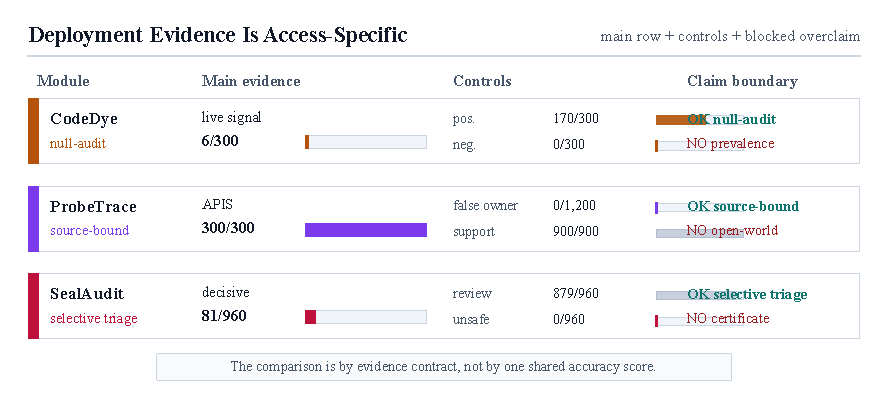
\includegraphics[width=\textwidth]{fig/blackbox_outcomes.pdf}
  \caption{Deployment-facing evidence contracts for sparse audit, scoped attribution, and selective triage. These are access-specific result surfaces, not comparable detector accuracies.}
  \label{fig:blackbox-outcomes}
\end{figure}

Figure~\ref{fig:blackbox-outcomes} makes the deployment contrast visible. CodeDye has low live yield, but positive and negative controls show that the audit predicate is not arbitrary. ProbeTrace is numerically strong because the owner registry and source split are fixed. SealAudit is intentionally abstention-heavy: most cases are routed to review, while unsafe pass-through remains the protected failure mode.

\begin{figure}[htbp]
  \centering
  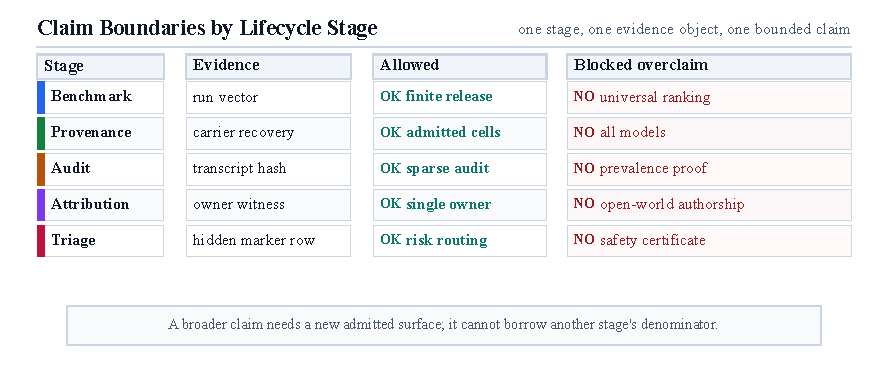
\includegraphics[width=\textwidth]{fig/claim_boundary_matrix.pdf}
  \caption{Claim boundaries across the lifecycle. The blocked-overclaim column is part of the method, not a footnote.}
  \label{fig:claim-boundary-matrix}
\end{figure}
\FloatBarrier

Figure~\ref{fig:claim-boundary-matrix} states the same rule visually. Every stage has an evidence object, an allowed reading, and a blocked overclaim. If later work adds a model family, provider, owner setting, or triage rule, it should create a new denominator rather than silently expanding the old one.

The two figures should therefore be read as complements rather than as repeated summaries. Figure~\ref{fig:blackbox-outcomes} shows why the three deployment-facing modules are not comparable by raw success rate: their rows represent different events. Figure~\ref{fig:claim-boundary-matrix} then records the stronger governance rule: a claim is admissible only inside the stage whose evidence object produced it. This is the synthesis contribution of WatermarkScope. The framework is not a weighted average of five systems; it is a set of constraints for deciding which result is allowed to mean what.

\section{Lessons Across Access Models}

The benchmark lesson is that executable evaluation changes the meaning of a watermark score. CodeMarkBench reports 140/140 canonical run completion, but that number is an inventory-completion result, not detector success. The scientific content is in component behavior: robustness, utility, release completeness, negative controls, and efficiency. This discipline carries into the later modules: SemCodebook keeps its 658 miss, abstain, or reject outcomes inside the positive denominator; CodeDye keeps no-signal rows inside the live audit denominator; ProbeTrace does not treat 900 transfer rows as primary APIS attributions; and SealAudit reports needs-review outcomes rather than hiding them behind accuracy.

The access-model lesson is that confidence cannot be transferred across stages. Under white-box access, SemCodebook can inspect typed carriers, validate helper closure, and recover an identifier with ECC-style decoding, schedule commitments, and positive-support evidence. Under black-box provider access, CodeDye cannot recover the same evidence object, so it preserves transcript-bound audit evidence instead. Under an owner-registry setting, ProbeTrace can make a stronger source-bound claim, but only because the active owner and source split are fixed before evaluation. Under security triage, SealAudit gives up broad classification coverage in exchange for an explicit unsafe-pass boundary.

The governance lesson is that watermarking systems need reviewable evidence, not only automatic labels. CodeDye is useful even with a sparse signal because it preserves rows for review without making an accusation. ProbeTrace distinguishes source-bound attribution from generic similarity. SealAudit turns ambiguous cases into explicit review work instead of forcing labels. These choices do not maximize one metric, but they avoid unsupported conclusions.

\section{Validity and Reproducibility}

Every rate in the dissertation is reported with a numerator, denominator, and claim boundary. For zero-event controls, the correct interpretation is not zero risk; it is 0 observed events with a nonzero upper confidence bound. For example, SemCodebook's 0/48,000 negative-control hits support a tight false-positive bound within the evaluated surface, while ProbeTrace's 0/1,200 false-owner controls support only the scoped owner protocol. For clustered evidence, such as ProbeTrace transfer rows, the primary independence unit remains the task cluster rather than the raw row count.

The principal internal-validity risk is outcome-dependent selection. The dissertation addresses it by separating claim-bearing rows from support-only rows and by recording denominator boundaries in manifests. The principal external-validity risk is that future models, providers, languages, attacks, or owner settings may behave differently. The response is denominator continuity: new model cells, providers, owner registries, or triage reruns should create new result surfaces rather than silently broadening the submitted FYP claims. The principal construct-validity risk is using the wrong metric for the question. Accuracy is not the right metric for SealAudit because abstention is designed; a weighted score is not the right metric for the lifecycle because recovery, audit yield, attribution, and triage coverage are different constructs.

The submitted code package supports this interpretation. The examiner-facing scripts verify that written claims are traceable to preserved result manifests, canonical artifacts, and claim-boundary files. They do not require a full GPU/API rerun inside the dissertation build. The report therefore separates three reproducibility layers: executable reruns for benchmark and local code, artifact reconstruction for preserved experiment outputs, and audit traceability for black-box transcripts or adjudicated rows.

The same separation explains the future-work plan. A new SemCodebook model family should not modify the reported 24,000-positive denominator; it should create a new admitted-cell surface. A new CodeDye provider should not be merged into the 300 DeepSeek rows; it should receive a provider-specific frozen audit surface and control suite. A future ProbeTrace multi-owner setting should add simultaneous-owner margins and owner-heldout controls before claiming broader attribution. A future SealAudit resolver should improve coverage only if it preserves the unsafe-pass event definition. These continuation rules are operational safeguards against overfitting because they prevent a later successful slice from rewriting the original denominator.

\section{Conclusion}

The research question asked how source-code watermarking can be evaluated, embedded, traced, and audited under realistic code-generation conditions. WatermarkScope answers it as an evidence chain: executable benchmarks expose reliability gaps, structured carriers support white-box provenance, black-box and owner-bound protocols preserve traceable evidence, and security triage audits marker-hidden risk. The completed FYP contribution is a benchmark-to-audit framework with code, artifacts, reproducible manifests, and conservative statistical reporting. Its central result is the evidence contract: as access weakens and risk changes, the claim must change with the evidence object.

The practical standard left by the dissertation is simple: future experiments should add denominators rather than quietly broadening old claims. A benchmark paper can expand CodeMarkBench with a new versioned matrix; a SemCodebook paper can admit new model cells; CodeDye can add provider-specific frozen controls; ProbeTrace can broaden registered owner surfaces; and SealAudit can improve coverage while preserving unsafe-pass accounting. These continuations are separated in Appendix~\ref{app:publication-plan}, but they share one rule: source-code watermarking becomes scientifically useful only when evidence, access, risk, and abstention are reported together.

For that reason, the final artifact should be judged as an evidence framework rather than as a collection of isolated prototypes. Its contribution is the combination of executable benchmarking, structured provenance, black-box audit preservation, source-bound attribution, and selective security triage under one reproducibility discipline. The strongest future version of the work is not obtained by making every number look larger; it is obtained by admitting new surfaces before measuring them, keeping weak or ambiguous outcomes visible, and letting the claim boundary change whenever access or risk changes.


\clearpage
\phantomsection
\addcontentsline{toc}{chapter}{References}
\begingroup
\sloppy
\emergencystretch=2em
\bibliographystyle{IEEEtran}
\bibliography{reference}
\endgroup

\clearpage
\phantomsection
\addcontentsline{toc}{chapter}{Appendices}
\appendix
\suppressappendixsubtoc
\appendixchapter{Code Repository and Artifact Access}{app:repository-access}

This appendix begins with repository access because the dissertation is a design project with implementation artifacts, not only a written report. The primary submitted FYP repository is:

\begin{center}
\href{https://github.com/Haoyi-Zhang/WatermarkScope}{\textnormal{https://github.com/Haoyi-Zhang/WatermarkScope}}
\end{center}

This is the repository to inspect for marking. It contains the dissertation source, the final PDF, implementation snapshots for the five stages, result manifests, claim-boundary files, and verification scripts. CodeMarkBench is also listed because it is the earlier benchmark artifact that supplies the executable foundation for the first lifecycle stage:

\begin{center}
\href{https://github.com/Haoyi-Zhang/CodeMarkBench}{\textnormal{https://github.com/Haoyi-Zhang/CodeMarkBench}}
\end{center}

\begin{table}[htbp]
\centering
\caption{Primary repository entry points for examiner inspection.}
\label{tab:repository-entry-points}
\lookuptable
\begin{tabularx}{\textwidth}{@{}L{2.35cm}YY@{}}
\toprule
Entry point & Contents & Examiner use \\
\midrule
Overview & Repository layout, headline results, project roles, and quick checks. & Start with the README before inspecting code or results. \\
Report source & Final PDF, LaTeX source, figures, bibliography, and appendices. & Verify that the submitted report is reproducible from source. \\
Project code & Code snapshots for CodeMarkBench, SemCodebook, CodeDye, ProbeTrace, and SealAudit. & Inspect implementation rather than relying only on prose. \\
Result records & Claim-bearing artifacts, compact summaries, and project reproducibility manifests. & Trace reported numbers to preserved evidence. \\
Claim manifest & Machine-readable claim-to-artifact binding with paths, hashes, denominators, and intervals. & Check whether a paper claim has a concrete artifact source. \\
Examiner check & Supervisor/examiner verification entry point. & Run local integrity checks without GPU or API access. \\
\bottomrule
\end{tabularx}
\end{table}

The concrete files corresponding to these entries in the primary FYP repository are \artifact{README.md},
\artifact{dissertation/}, \artifact{projects/}, \artifact{results/},
\artifact{RESULT\_MANIFEST.jsonl}, and
\artifact{scripts/examiner\_check.py}. They are named in prose instead of
being forced into narrow table cells so that the printed appendix remains
readable.

The WatermarkScope repository is intentionally not a raw dump of every temporary run. Large raw provider outputs and full-scale continuation artifacts are kept out of the review mirror when they are not needed for ordinary marking. Their role is represented by manifests, compact claim-bearing artifacts, and reproducibility notes. This keeps the submitted code package inspectable while preserving the distinction between local integrity checks and full GPU/API reruns. The separate CodeMarkBench repository should be read as public benchmark infrastructure and future publication material; the FYP submission itself is the WatermarkScope repository above.

\begin{table}[htbp]
\centering
\caption{Five-stage code layout in the submitted repository.}
\label{tab:repository-stage-layout}
\lookuptable
\begin{tabularx}{\textwidth}{@{}L{2.05cm}L{2.65cm}Y@{}}
\toprule
Stage & Code path & Main inspection target \\
\midrule
Benchmark & CodeMarkBench & Benchmark harness, release tables, source groups, and baseline adapters. \\
Provenance & SemCodebook & Structured carrier recovery implementation, scripts, tests, and white-box evidence gates. \\
Audit & CodeDye & Frozen black-box null-audit protocol, controls, and support-row exclusions. \\
Attribution & ProbeTrace & Active-owner attribution scripts, control gates, and transfer-binding artifacts. \\
Triage & SealAudit & Marker-hidden triage resolver, safety-boundary scripts, and coverage-risk artifacts. \\
\bottomrule
\end{tabularx}
\end{table}

All five stage folders are stored under the top-level \artifact{projects/}
directory. The table uses stage names rather than full path strings to keep
the appendix compact; the directory names match the submitted repository.

For a fast local check, run:
\begin{center}
\artifact{python scripts/examiner\_check.py}
\end{center}
This command checks the repository structure, manifest consistency, preserved-result hashes, headline denominators, confidence-interval metadata, and required project snapshots. It is not a full rerun of all model or provider experiments; full reruns require model weights, GPU resources, or live API access depending on the module.

\appendixchapter{Evidence Contract and Manifest}{app:artifact-index}

This appendix is an examiner-facing evidence contract. It does not repeat the dissertation as five mini-projects. Instead, it records how the lifecycle stages in the main body map to notation, code snapshots, result artifacts, and claim boundaries. The machine-readable binding is in \artifact{RESULT\_MANIFEST.jsonl}.

\section{Lifecycle Notation}

Table~\ref{tab:lifecycle-notation-summary-app} expands Eq.~\ref{eq:lifecycle-stage}. The key point is that every stage has both an allowed interpretation and a forbidden interpretation.

\begin{table}[htbp]
\centering
\caption{Evidence-contract notation used across the dissertation.}
\label{tab:lifecycle-notation-summary-app}
\tighttable
\begin{tabularx}{\textwidth}{@{}L{1.55cm}Y@{}}
\toprule
Symbol & Meaning \\
\midrule
$\mathcal{L}_j$ & Lifecycle stage $j$: benchmark, provenance, audit, attribution, or triage. \\
$\mathcal{A}_j$ & Access model: local white-box model, black-box provider, owner registry, or marker-hidden audit setting. \\
$\mathcal{O}_j$ & Evidence object: run record, carrier recovery, transcript hash, owner witness, or triage row. \\
$\mathcal{D}_j$ & Fixed denominator for the main claim at that stage. \\
$\mathcal{C}_j$ & Control set, including negative controls, false-owner controls, marker-hidden controls, or support-row exclusions. \\
$\delta_j$ & Frozen decision rule or resolver used before result interpretation. \\
$\mathcal{M}_j$ & Reported metric vector, including rates, intervals, bounds, costs, and abstentions when relevant. \\
$\mathcal{I}_j$ & Allowed interpretation supported by the claim-bearing denominator. \\
$\mathcal{F}_j$ & Forbidden interpretation, such as universal watermarking, prevalence, provider-general authorship, or safety certification. \\
\bottomrule
\end{tabularx}
\end{table}

\section{Statistical Reporting Rules}

For a result with $k$ observed events over $n$ claim-bearing records, the observed rate is $\hat{p}=k/n$. The Wilson interval used in the main tables is computed with $z=1.96$:
\begin{align}
  c &= \frac{\hat{p}+z^2/(2n)}{1+z^2/n},&
  h &= \frac{z\sqrt{\hat{p}(1-\hat{p})/n+z^2/(4n^2)}}{1+z^2/n},
\end{align}
and reported as $[c-h,c+h]$. Zero-event rows are reported as ``0 observed'' plus the upper interval endpoint, not as zero risk. These are descriptive binomial row-level intervals over the submitted denominators. Clustered or repeated rows require the separately reported independence unit and should not be read as fully independent future-task inference.

\begin{table}[htbp]
\centering
\caption{Rules used to keep result reporting conservative.}
\label{tab:stat-reporting-rules}
\tighttable
\begin{tabularx}{\textwidth}{@{}L{2.25cm}YY@{}}
\toprule
Case & Reporting rule & Reason \\
\midrule
Ordinary binomial rate & Report $k/n$ and Wilson-style 95\% interval. & Avoids naked percentages. \\
Zero-event result & Report 0 observed and a nonzero upper bound. & Avoids implying zero mathematical risk. \\
Perfect observed result & Report lower confidence bound. & Avoids absolute-certainty wording. \\
Clustered rows & State the primary independence unit. & Avoids inflated support surfaces. \\
Support-only rows & Exclude from main denominators. & Prevents post-hoc denominator drift. \\
\bottomrule
\end{tabularx}
\end{table}

\section{Claim-Row Schema}

\begin{table}[htbp]
\centering
\caption{Shared claim-row field groups.}
\label{tab:claim-row-fields-app}
\tighttable
\begin{tabularx}{\textwidth}{@{}L{2.20cm}Y@{}}
\toprule
Field group & Purpose \\
\midrule
Identity & Task/case identifier, language, source group, and model/provider/owner context. \\
Hash binding & Prompt, raw payload, and structured payload hashes for later inspection. \\
Version binding & Detector version, threshold version, baseline/control name, and attack condition. \\
Decision evidence & Decision, score/support statistic, and abstain reason when applicable. \\
Claim boundary & Claim-bearing flag and support-only exclusion reason. \\
\bottomrule
\end{tabularx}
\end{table}

\begin{table}[htbp]
\centering
\caption{Main artifact families used by the dissertation. Exact paths and hashes are bound in \artifact{RESULT\_MANIFEST.jsonl}.}
\label{tab:appendix-artifact-index}
\tighttable
\begin{tabularx}{\textwidth}{@{}L{1.80cm}L{2.45cm}YY@{}}
\toprule
Lifecycle stage & Artifact family & Evidence supported & Boundary \\
\midrule
Benchmark & Benchmark tables & Run inventory, method leaderboard, robustness--utility summary & Finite release matrix \\
Provenance & White-box gates & 72,000-row surface, positive/negative records, ablation gate & Admitted cells only \\
Audit & Null-audit gates & 300 live rows, positive/negative controls, support-row exclusion & Null audit only \\
Attribution & Owner evidence & APIS-300 evidence, false-owner controls, transfer receipts & Single active owner \\
Triage & Risk gates & Marker-hidden triage rows, coverage-risk frontier, resolver gate & Selective triage \\
\bottomrule
\end{tabularx}
\end{table}

\section{How To Read The Manifest}

The repository intentionally keeps long file paths out of the main-body tables. A reader should use \artifact{RESULT\_MANIFEST.jsonl} as the lookup layer: each row contains the relative path, SHA-256 hash, module, claim text, numerator, denominator, independence unit, and boundary. This keeps the appendix readable while preserving exact artifact traceability.

\section{Manifest Fields}

Each manifest row stores a relative artifact path, SHA-256 hash, module name, claim text, numerator, denominator, independence unit when applicable, confidence-interval metadata when required, and a prose boundary. This allows a reader to start from a table in the dissertation, locate the exact artifact, verify the hash, and recover the reported denominator.

\begin{table}[htbp]
\centering
\caption{Manifest field definitions.}
\label{tab:manifest-field-definitions}
\tighttable
\begin{tabularx}{\textwidth}{@{}L{2.25cm}L{1.55cm}Y@{}}
\toprule
Field & Required & Examiner use \\
\midrule
\artifact{path} & yes & Locate the artifact relative to the package root. \\
\artifact{sha256} & yes & Verify the exact file used by the report. \\
\artifact{module} & yes & Connect the artifact to the lifecycle stage. \\
\artifact{claim} & yes & Identify the supported result or boundary. \\
\artifact{num.}/\artifact{denom.} & when applicable & Recover the reported rate. \\
\artifact{indep. unit} & when applicable & Detect clustering or repeated-row issues. \\
\artifact{ci95\_low}, \artifact{ci95\_high} & for CI-bearing rows & Verify uncertainty wording. \\
\artifact{boundary} & yes & Check that the artifact does not support a broader claim. \\
\bottomrule
\end{tabularx}
\end{table}

\begin{table}[htbp]
\centering
\caption{Lifecycle-level repository lookup.}
\label{tab:repo-lookup}
\lookuptable
\begin{tabularx}{\textwidth}{@{}L{1.45cm}L{2.25cm}L{2.25cm}Y@{}}
\toprule
Layer & Code family & Result family & Examiner question answered \\
\midrule
Benchmark & Benchmark code & Benchmark results & Are benchmark tasks, baselines, and run tables present? \\
Provenance & SemCodebook code & SemCodebook results & Are carrier recovery, negative controls, and ablation gates bound? \\
Audit & CodeDye code & CodeDye results & Are live rows, controls, and support-row exclusions separated? \\
Attribution & ProbeTrace code & ProbeTrace results & Are owner controls and transfer receipts scoped correctly? \\
Triage & SealAudit code & SealAudit results & Are hidden-row coverage and unsafe-pass boundaries explicit? \\
\bottomrule
\end{tabularx}
\end{table}

\section{Support-Only Rule}

Rows produced for diagnostics, canaries, stress exploration, old release surfaces, or support examples may remain useful for engineering review, but they do not enter the main denominator unless the manifest marks them as claim-bearing before interpretation. This rule is the main protection against retrofitting an attractive result after seeing outcomes.

\begin{table}[htbp]
\centering
\caption{Support-only surfaces retained for auditability but excluded from main claims.}
\label{tab:support-only-ledger}
\tighttable
\begin{tabularx}{\textwidth}{@{}L{2.10cm}L{1.45cm}YY@{}}
\toprule
Surface & Count & Role & Must not be used as \\
\midrule
SemCodebook ablation & 43,200 & Method-support surface for component interventions. & Main recovery denominator or unsupported causal effect table. \\
CodeDye support rows & 806 & Public/support/stress auditability evidence. & Live DeepSeek audit denominator. \\
CodeDye stats sub-gate & 4/300 & Narrow reproducibility sub-definition. & Replacement for the 6/300 reporting signal. \\
ProbeTrace transfer & 900 & Source-bound support over 300 task clusters. & 900 independent attribution tasks. \\
SealAudit marker-visible & 320 & Diagnostic visibility surface. & Marker-hidden claim denominator. \\
\bottomrule
\end{tabularx}
\end{table}

\section{Lifecycle Evidence Ledger}

Table~\ref{tab:lifecycle-evidence-ledger} gives a compact reading ledger for the five lifecycle stages. It is intended for examiners who want to move from a main-body number to the corresponding evidence discipline without reading every artifact file. The table deliberately lists the primary denominator, the principal control, the allowed conclusion, and the most likely overclaim.

\begin{table}[htbp]
\centering
\caption{Lifecycle evidence ledger for examiner reading.}
\label{tab:lifecycle-evidence-ledger}
\tighttable
\begin{tabularx}{\textwidth}{@{}L{1.65cm}L{2.25cm}L{2.25cm}YY@{}}
\toprule
Stage & Primary denominator & Principal control & Allowed conclusion & Most likely overclaim \\
\midrule
Benchmark & 140 canonical model-method-source runs & Clean controls and executable attack rows & Existing baselines show multidimensional tradeoffs. & Ranking every possible method or model. \\
Provenance & 24,000 positives and 48,000 negatives & Negative controls and admitted-cell gates & Structured carriers can recover provenance in admitted white-box cells. & Universal semantic watermarking. \\
Audit & 300 live rows plus frozen controls & Positive and negative contamination controls & Sparse null-audit evidence is preserved honestly. & Provider contamination prevalence. \\
Attribution & 300 APIS rows plus 1,200 controls & Owner controls & Single-active-owner source binding is supported. & Open-world authorship attribution. \\
Triage & 960 marker-hidden rows & Unsafe-pass accounting and diagnostic visible rows & Conservative triage routes ambiguity to review. & Automatic security certification. \\
\bottomrule
\end{tabularx}
\end{table}

The ledger is useful because it separates evidence quantity from claim strength. A large denominator can still support a narrow claim if the access model is narrow. A perfect observed rate can still be scoped if the evaluated owner, provider, or marker setting is scoped. A low decisive coverage can still be useful if the intended output is triage rather than forced classification. These distinctions are exactly what the main body means by a denominator-aware framework.

\section{Examiner Claim Checklist}

The following checklist is the shortest way to audit a result table. A row is not claim-bearing because it appears in a CSV file; it is claim-bearing only when the denominator, control role, version, and boundary are fixed before interpretation.

\begin{table}[htbp]
\centering
\caption{Checklist used to decide whether a row can support a main claim.}
\label{tab:examiner-claim-checklist}
\tighttable
\begin{tabularx}{\textwidth}{@{}L{2.10cm}YY@{}}
\toprule
Check & Pass condition & If the check fails \\
\midrule
Identity binding & Task, case, model/provider/owner, and source group are fixed. & Row is diagnostic or support-only. \\
Version binding & Detector, threshold, prompt template, and parser versions are recorded. & Row cannot be merged into a main denominator. \\
Control role & Positive, negative, false-owner, diagnostic, or support role is declared. & Row is not interpretable as evidence. \\
Outcome independence & Admission does not depend on detector score or observed label. & Row is excluded from claim-bearing tables. \\
Hash or artifact binding & Raw/structured payload or result artifact has a stable digest. & Row remains unverifiable support. \\
Boundary statement & Allowed and forbidden readings are written near the result. & Result is unsafe for main-body use. \\
\bottomrule
\end{tabularx}
\end{table}

This checklist also explains why the dissertation keeps some apparently useful rows out of the main claims. A support row may have complete hashes and may even look persuasive, but if it was generated for debugging, canary tuning, visibility diagnosis, or old-release comparison, it cannot be promoted after its outcome is known. This rule is stricter than many informal project reports, but it makes the evidence surface easier to defend.

\section{Manifest-To-Text Traceability}

Table~\ref{tab:manifest-to-text-traceability} gives the reading order used when checking a claim from prose back to artifacts. The table avoids long repository paths in print; exact relative paths are stored in the manifest and are better inspected in a text editor or script output than in a narrow PDF column.

\begin{table}[htbp]
\centering
\caption{Traceability path from dissertation statement to released evidence.}
\label{tab:manifest-to-text-traceability}
\tighttable
\begin{tabularx}{\textwidth}{@{}L{2.15cm}YY@{}}
\toprule
Reader action & Artifact discipline & Why it matters \\
\midrule
Start from a result sentence & Identify the lifecycle stage and denominator named in the sentence. & Prevents using a nearby but different result surface. \\
Open the main table source & Confirm numerator, denominator, control role, and excluded rows. & Separates claim-bearing rows from support-only rows. \\
Check the manifest entry & Verify module name, digest, and boundary text. & Connects prose to a stable file rather than memory. \\
Read the boundary file & Compare allowed and forbidden interpretations. & Catches overclaiming before publication writing. \\
Run the examiner check & Confirm local package integrity and stale-wording gates. & Provides a one-command sanity check for the submitted package. \\
\bottomrule
\end{tabularx}
\end{table}

This traceability path is intentionally more formal than a typical FYP appendix. It makes the report easier to audit because an examiner can challenge a number without reverse-engineering the whole repository. If a future manuscript changes a denominator, the corresponding manifest row must change too; otherwise the old FYP text remains the authoritative claim boundary.

\section{Lifecycle Dependency Map}

The five stages form a dependency chain. CodeMarkBench is not only a background benchmark; it establishes the execution and denominator discipline used by every later module. SemCodebook depends on that discipline to report structured recovery without deleting misses. CodeDye depends on SemCodebook's access-model distinction to explain why black-box evidence is transcript-bound. ProbeTrace depends on the audit record idea but adds an owner registry. SealAudit depends on all earlier stages because safety triage only makes sense after the evidence object is explicit.

\begin{table}[htbp]
\centering
\caption{How each lifecycle stage constrains the next stage.}
\label{tab:lifecycle-dependency-map}
\tighttable
\begin{tabularx}{\textwidth}{@{}L{1.85cm}YY@{}}
\toprule
Stage & Constraint inherited by the next stage & Failure if ignored \\
\midrule
Benchmark & Count only executable and release-bound evidence. & Later method claims inherit unstable denominators. \\
Provenance & Preserve misses, abstentions, and negative controls. & White-box recovery appears stronger than it is. \\
Audit & Keep black-box transcripts hash-bound and scoped. & Sparse signals become unsupported prevalence claims. \\
Attribution & Require owner and source-split commitments. & Similarity evidence becomes open-world authorship. \\
Triage & Treat ambiguity as a first-class output. & Safety evidence becomes a misleading classifier score. \\
\bottomrule
\end{tabularx}
\end{table}

This dependency map is the compact version of the dissertation story. It is also a practical checklist for later paper writing: a future paper may focus on one stage, but it should not discard the constraint inherited from the previous stage.

\appendixchapter{Supplementary Methods and Reproducibility}{app:reproducibility}

This appendix gives the compact technical lookup material that would be too detailed for the main body. It is organized by evidence function rather than by project folder so that the dissertation remains one framework.

\section{Notation Summary}

\begin{table}[htbp]
\centering
\caption{Core notation used across the dissertation.}
\label{tab:notation-summary}
\tighttable
\begin{tabularx}{\textwidth}{@{}L{1.95cm}Y@{}}
\toprule
Symbol & Meaning \\
\midrule
$\mathcal{B}$ & CodeMarkBench tuple of tasks, source groups, models, watermark methods, attacks, and evaluators. \\
$\mathcal{T}_s$ & Executable task slice for source group $s$; $\mathcal{T}=\bigsqcup_s\mathcal{T}_s$. \\
$C_r(x)$ & Carrier set extracted from representation family $r\in\{\mathrm{AST},\mathrm{CFG},\mathrm{SSA}\}$. \\
$\rho_i,\ell_{i,j}$ & Keyed carrier family and slot selected for encoded bit position $i$ and retry counter $j$. \\
$\kappa$ & SemCodebook schedule digest over payload, adaptive schedule, and detector version. \\
$r_i$ & Shared claim-row record in Eq.~\ref{eq:claim-row}. \\
$b_i$ & Claim-bearing flag; only rows with $b_i=1$ may enter a main denominator. \\
$\hat{p}$ & Observed rate $k/n$ over a fixed denominator. \\
$\tau$ & Frozen threshold version used by a detector or audit protocol. \\
$\hat{y}_i$ & SealAudit triage decision for marker-hidden row $i$. \\
\bottomrule
\end{tabularx}
\end{table}
\FloatBarrier

\section{Supplementary Method Details}

\begin{table}[htbp]
\centering
\caption{Supplementary method details by evidence function.}
\label{tab:supplementary-method-details}
\tighttable
\begin{tabularx}{\textwidth}{@{}L{2.25cm}YY@{}}
\toprule
Evidence function & Include in examiner reading & Keep out of main claims \\
\midrule
Executable benchmark contract & Run/task denominator distinction, metric vector, negative controls, release stability. & Full leaderboard dumps or unsupported winner-takes-all ranking. \\
Structured provenance & AST/CFG/SSA-style carrier summary, adaptive schedule commitments, ECC-style recovery, admission rules, failure accounting. & Raw 72,000-row listings or no-retry overclaims. \\
Black-box audit & Hash-retention record, 6/300 versus 4/300 boundary, support-row exclusion. & Provider transcript raw text or prevalence estimates. \\
Source attribution & Registry object, APIS denominator, false-owner controls, transfer-cluster rule. & Treating 900 transfer rows as 900 primary tasks. \\
Selective triage & Marker-hidden denominator, needs-review semantics, unsafe-pass event definition. & Marker-visible diagnostics as the main result. \\
\bottomrule
\end{tabularx}
\end{table}
\FloatBarrier

\section{Benchmark Metric Details}

For a fixed method, model, and source group, utility is reported over the executable task slice:
\begin{equation}
  \widehat{U}(w,m,s)=
  \frac{1}{|\mathcal{T}_s|}
  \sum_{t\in\mathcal{T}_s} U(G(m,t,w)).
\end{equation}
For a fixed watermark method and attack, the finite-sample robustness estimator is
computed over the released admitted watermarked set $\mathcal{X}_w$ and the matched
admitted unwatermarked control set $\mathcal{X}_0$:
\begin{equation}
  \widehat{\mathrm{RobustTPR}}(w,a)=
  \frac{\sum_{x\in\mathcal{X}_w}\mathbf{1}[V_{\mathrm{attack}}(A_a(x))=1\wedge D_w(A_a(x))=1]}
       {\sum_{x\in\mathcal{X}_w}\mathbf{1}[V_{\mathrm{attack}}(A_a(x))=1]}.
\end{equation}
The corresponding control estimator is computed over unwatermarked rows:
\begin{equation}
  \widehat{\mathrm{FPR}}(w,a)=
  \frac{\sum_{x_0\in\mathcal{X}_0}\mathbf{1}[V_{\mathrm{attack}}(A_a(x_0))=1\wedge D_w(A_a(x_0))=1]}
       {\sum_{x_0\in\mathcal{X}_0}\mathbf{1}[V_{\mathrm{attack}}(A_a(x_0))=1]}.
\end{equation}
Generation overhead is reported as a matched aggregate over the same admitted task slice:
\begin{equation}
  \mathrm{Overhead} =
  \frac{\sum_i \mathrm{time}_{\mathrm{watermarked}}(i)-\sum_i \mathrm{time}_{\mathrm{baseline}}(i)}
       {\sum_i \mathrm{time}_{\mathrm{baseline}}(i)}.
\end{equation}

\begin{table}[htbp]
\centering
\caption{CodeMarkBench component-vector definitions. These fields explain the released method table; they are not independent pass/fail gates.}
\label{tab:codemarkbench-components-app}
\tighttable
\begin{tabularx}{\textwidth}{@{}L{1.90cm}L{2.20cm}Y@{}}
\toprule
Component & Direction & Meaning in the release table \\
\midrule
$q_{\mathrm{core}}$ & larger is better & Detector behavior on core transformations and standard admitted rows. \\
$q_{\mathrm{robust}}$ & larger is better & Detection retained under executable attacks that preserve program validity. \\
$q_{\mathrm{utility}}$ & larger is better & Pass-rate preservation for generated artifacts under the executable harness. \\
$q_{\mathrm{gate}}$ & larger is better & Release-completeness and implementation-admission component, not a binary accept decision. \\
$q_{\mathrm{negFPR}}$ & larger is better & Inverted negative-control false-positive behavior; raw false-positive rates remain printed separately. \\
$q_{\mathrm{efficiency}}$ & larger is better & Normalized generation/evaluation overhead where available in the release surface. \\
\bottomrule
\end{tabularx}
\end{table}
\FloatBarrier

\section{Protocol Pseudocode}

\begin{algorithm}[!htbp]
\caption{SemCodebook Embed Protocol}
\label{alg:semcodebook}
\begin{algorithmic}[1]
\Require Task identifier $t$, code artifact $x$, secret key $K$, provenance identifier $\mathrm{id}$
\State Extract tagged carriers $C(x)$ from AST, CFG, and SSA families
\If{$|C(x)|=0$ or typed carrier coverage is below threshold}
  \State \Return abstain if row is already admitted; otherwise record nonpromotion
\EndIf
\State Score carrier families by applicability, frozen family bias, and HMAC-derived tie-break
\State Build adaptive data-slot and anchor-slot schedule plus public schedule commitment record
\State Encode payload bits with the configured ECC-style schedule block
\For{each encoded position $i$}
  \State Select unused carrier slot by keyed schedule with collision retry
  \If{the selected family has no admissible carrier}
    \State \Return abstain
  \ElsIf{collision retry budget is exhausted}
    \State \Return abstain
  \EndIf
  \State Materialize the scheduled carrier without breaking executable behavior
  \If{materialization breaks parse or executable validation}
    \State \Return materialization\_failure counted in the admitted denominator
  \EndIf
\EndFor
\State \Return watermarked artifact and public schedule digest record
\end{algorithmic}
\end{algorithm}

\begin{algorithm}[!htbp]
\caption{SemCodebook Recover Protocol}
\label{alg:semcodebook-recover}
\begin{algorithmic}[1]
\Require Candidate code artifact $x'$, task identifier $t$, key $K$, schedule/recovery version $v_{\mathrm{sched}}$
\State Recompute admissible carrier families and adaptive keyed schedule
\If{carrier coverage is below threshold or support families are insufficient}
  \State \Return abstain
\EndIf
\State Extract observations $o_1,\ldots,o_L$ from scheduled carriers
\State Decode $\widehat{\mathrm{payload}}\gets \mathrm{ECC\_Decode}(o_1,\ldots,o_L)$
\If{ECC check fails, payload mismatches, or positive-support/schedule evidence fails}
  \State \Return reject
\Else
  \State \Return recovered identifier and verified support evidence
\EndIf
\end{algorithmic}
\end{algorithm}

\FloatBarrier

\begin{table}[!htbp]
\centering
\caption{Compact decision sketches for the black-box and deployment protocols. The shared admission logic is given in Algorithm~\ref{alg:evidence-admission}; this table records only the stage-specific decision rule.}
\label{tab:protocol-sketches}
\lookuptable
\begin{tabularx}{\textwidth}{@{}L{2.1cm}YY@{}}
\toprule
Protocol & Stage-specific decision rule & Failure accounting \\
\midrule
SemCodebook admission & Distinguish pre-run nonpromotion from post-admission recovery failures. & Missing model/parser/helper closure is nonpromotion; carrier insufficiency, ECC rejection, payload mismatch, support-gate failure, and materialization failure remain abstain/reject/failure inside the admitted positive denominator. \\
CodeDye frozen null-audit &
Store prompt, raw-response, and structured hashes; compute the frozen non-weighted gate vector over family observation, structural or stable witness evidence, output-visible canary evidence, and heldout/rewrite context; report a sparse signal only when the final evidence stage passes. &
Pre-admission failures remain diagnostic; post-admission no-signal rows stay inside the 300-row live denominator. \\
ProbeTrace single-owner attribution &
Compute active-owner witness score and same-task wrong/null/random-owner controls; attribute only when the active witness passes and all controls remain below their frozen thresholds. &
Low active evidence abstains; control violation rejects inside the APIS denominator; transfer rows remain support over task clusters. \\
SealAudit conservative triage &
Collect marker-hidden static, semantic, laundering, spoofability, and judge-perturbation evidence; return a decisive label only when evidence is sufficient and non-conflicting. &
Insufficient or conflicting evidence returns \needsreview; unsafe-pass is reported as a separate audit-error event, not hidden inside accuracy. \\
\bottomrule
\end{tabularx}
\end{table}

\FloatBarrier

\section{Admission And Boundary Tables}

\begin{table}[htbp]
\centering
\caption{SemCodebook admission rule for white-box claim cells.}
\label{tab:sem-admission-app}
\tighttable
\begin{tabularx}{\textwidth}{@{}L{2.25cm}YY@{}}
\toprule
Gate & Required condition & If condition fails \\
\midrule
Model admission & Frozen local code-model revision and scale bucket & Nonpromotion audit; no main claim \\
Execution admission & Source group has executable tests and attack harness & Support-only diagnostic \\
Carrier admission & AST/CFG/SSA extractor available before run; row-level typed coverage checked after admission & Pre-run extractor absence is nonpromotion; row-level insufficiency is abstain inside denominator \\
Closure admission & Helpers, imports, package prelude, and transitive calls validated before run & Missing closure is nonpromotion; post-admission materialization/compiler failure is counted failure \\
\bottomrule
\end{tabularx}
\end{table}

\section{Examiner Verification Entry Points}

The submitted repository preserves the dissertation PDF, code snapshots, result artifacts, hash manifest, and verification scripts. The main entry points are:
\begin{itemize}
  \item \artifact{dissertation/WatermarkScope\_FYP\_Dissertation.pdf}: submitted report;
  \item \artifact{RESULT\_MANIFEST.jsonl}: claim-to-artifact binding with hashes;
  \item \artifact{CLAIM\_BOUNDARIES.md}: allowed and forbidden interpretations;
  \item \artifact{scripts/repro\_check.py}: repository integrity, stale wording, hash, and denominator checks;
  \item \artifact{scripts/examiner\_check.py}: one-command examiner-facing check;
  \item \href{https://github.com/Haoyi-Zhang/WatermarkScope}{WatermarkScope}: submitted FYP repository with dissertation source, method snapshots, manifests, and verification scripts;
  \item \href{https://github.com/Haoyi-Zhang/CodeMarkBench}{CodeMarkBench}: public benchmark repository and software artifact snapshot.
\end{itemize}

The local verification layer has a narrow examination purpose: it checks that the submitted claims still bind to preserved artifacts, that support-only rows are not promoted, and that no stale internal material has entered the examiner-facing package.

\begin{table}[htbp]
\centering
\caption{Local examiner checks and the evidence risk each one targets.}
\label{tab:local-examiner-checks}
\tighttable
\begin{tabularx}{\textwidth}{@{}L{2.35cm}YY@{}}
\toprule
Check family & Targeted risk & Expected reading \\
\midrule
Package integrity & Missing source snapshots, result artifacts, manifests, or examiner documents. & The dissertation can be inspected without private working files. \\
Claim reconstruction & A printed numerator or denominator no longer matches the manifest. & Each headline number has a preserved artifact path and digest. \\
Boundary lint & Support rows, diagnostics, or historical blockers enter main claims. & Reviewer-facing text keeps allowed and forbidden interpretations separate. \\
Secret and stale scan & API tokens, private paths, cache files, failed drafts, or temporary logs leak into the package. & The package is clean enough for supervisor/examiner sharing. \\
Preservation audit & Existing result artifacts are silently modified during writing. & Preserved experiment outputs remain immutable unless a new result row is explicitly added. \\
\bottomrule
\end{tabularx}
\end{table}
\FloatBarrier

\section{Reproducibility Tiers}

\begin{table}[htbp]
\centering
\caption{What each reproducibility tier proves.}
\label{tab:reproducibility-tiers}
\tighttable
\begin{tabularx}{\textwidth}{@{}L{1.75cm}L{2.15cm}YY@{}}
\toprule
Tier & Command or artifact & What it proves & What it does not prove \\
\midrule
Local package check & examiner check & Files, hashes, denominators, stale wording, and manifest consistency. & Full GPU/API experiment regeneration. \\
Manifest summary & summary script & Claim-to-artifact binding and result-surface summaries. & Model/provider reproducibility. \\
Code snapshot inspection & project snapshots & Implementations and scripts are present for examiner review. & All large experiments rerun on a normal laptop. \\
Full rerun & GPU/API access & Experimental regeneration under the recorded settings. & Feasibility within the submitted local check. \\
\bottomrule
\end{tabularx}
\end{table}

\section{Main-Body Result Reconstruction}

The dissertation's headline numbers can be reconstructed from the manifest rather than from prose alone. Table~\ref{tab:result-reconstruction-app} records the arithmetic used in the main body. The table is not intended to introduce new claims; it gives the denominator arithmetic in one place so that a reader can check that rates are not mixed across modules.

\begin{table}[htbp]
\centering
\caption{Reconstruction of main-body quantitative readings.}
\label{tab:result-reconstruction-app}
\tighttable
\begin{tabularx}{\textwidth}{@{}L{2.15cm}L{1.95cm}L{2.30cm}Y@{}}
\toprule
Result & Count & Reported reading & Boundary \\
\midrule
Benchmark inventory & 140/140 & Complete canonical run inventory. & Inventory completion, not detector success. \\
SCB recovery & 23,342/24k & 97.26\% recovered. & Admitted white-box positive denominator. \\
SemCodebook negative & 0/48,000 & No observed negative-control hit. & Nonzero upper bound still governs risk. \\
CodeDye live audit & 6/300 & Sparse 2.00\% live signal. & Null-audit signal, not prevalence. \\
CodeDye controls & 170/300; 0/300 & Positive sensitivity and clean negatives. & Calibration, not live denominator expansion. \\
ProbeTrace APIS & 300/300 & Scoped active-owner decisions promoted. & Single active owner only. \\
ProbeTrace controls & 0/1,200 & No observed false-owner hit. & Wrong/null/random controls only. \\
SealAudit triage & 81/960; 879/960 & Decisive and needs-review split. & Selective triage, not automatic classification. \\
SealAudit unsafe pass & 0/960 & No observed unsafe pass. & Marker-hidden rows only. \\
\bottomrule
\end{tabularx}
\end{table}

\section{Failure-Mode Interpretation}

The framework is designed so that failures remain scientifically useful. A failed executable attack in CodeMarkBench reveals a utility or transformation-boundary issue. A SemCodebook miss, abstain, or reject reveals carrier insufficiency, ECC failure, decoded-payload mismatch, or support-gate inconsistency. A CodeDye no-signal row says that the frozen non-weighted evidence stage did not fire, but not that related material was absent from training. A ProbeTrace abstention would indicate insufficient active-owner evidence rather than a negative authorship theorem. A SealAudit needs-review decision indicates that safety evidence is insufficient or conflicting.

\begin{table}[htbp]
\centering
\caption{How non-success outcomes are interpreted.}
\label{tab:failure-mode-interpretation}
\tighttable
\begin{tabularx}{\textwidth}{@{}L{2.15cm}L{2.35cm}YY@{}}
\toprule
Module & Non-success outcome & Counted as & Interpretation \\
\midrule
Benchmark & Non-executable transformed artifact & Attack utility boundary & The transformation cannot support robustness evidence. \\
SemCodebook & Miss, abstain, reject & Positive denominator outcome & Recovery failed or evidence was insufficient. \\
CodeDye & No live signal & Live denominator outcome & The frozen audit predicate did not fire. \\
ProbeTrace & Low active evidence or control violation & APIS denominator outcome & Attribution abstains or rejects under the scoped rule. \\
SealAudit & Needs review & Marker-hidden denominator outcome & Evidence is insufficient or conflicting for decisive triage. \\
\bottomrule
\end{tabularx}
\end{table}

This failure-mode interpretation is central to the dissertation's anti-overfitting stance. The easiest way to make a watermarking result look stronger is to remove inconvenient outcomes or merge support rows into a favorable denominator. WatermarkScope instead preserves non-success outcomes as evidence about where a method is strong, where it is fragile, and where the claim must be narrowed.

\section{Examiner Reproduction Walkthrough}

The repository is designed for two levels of examiner checking. The first level is a local integrity check: it verifies that the report, manifests, scripts, and preserved result files agree. The second level is a research reproduction check: it reruns selected experimental modules when GPU or API access is available. The submitted package does not require a full GPU/API rerun for basic marking, but it records the boundary between the two checks.

\begin{table}[htbp]
\centering
\caption{Recommended examiner walkthrough for the submitted package.}
\label{tab:examiner-walkthrough}
\tighttable
\begin{tabularx}{\textwidth}{@{}L{2.00cm}YY@{}}
\toprule
Step & What to inspect & Expected outcome \\
\midrule
Read README & Project story, folder map, and integrity command. & The package is understandable without private notes. \\
Open PDF & Main body, references, and appendices. & Claims match the manifest and do not exceed 40 main-body pages. \\
Run examiner check & Local files, stale wording, and manifest consistency. & No secret-like token, stale failed-run wording, or missing canonical artifact. \\
Inspect snapshots & Code for benchmark, provenance, audit, attribution, and triage modules. & The FYP contains code, not only result summaries. \\
Inspect result manifest & Claim text, denominator, digest, and boundary. & Each main result is traceable to a preserved artifact. \\
Optional rerun & Selected smoke or full experiment, depending on resources. & Rerun status is reported separately from submitted claim validity. \\
\bottomrule
\end{tabularx}
\end{table}

This walkthrough is intentionally examiner-facing rather than developer-facing. It avoids requiring a marker to read every intermediate file before understanding the project. At the same time, it leaves enough structure for a technical examiner to audit a number from the PDF back to a script, a manifest row, and a result artifact.

\section{Artifact Preservation Policy}

The submitted package preserves the evidence needed to understand the FYP, not every temporary file produced during development. Preserved artifacts satisfy at least one of three roles: they support a main result, explain a support-only exclusion, or allow an examiner to verify the dissertation. Generated caches, scratch logs, and private-path material are outside the evidence surface and are not part of the submitted record.

\begin{table}[htbp]
\centering
\caption{Evidence-preservation policy for the final submission package.}
\label{tab:artifact-preservation-policy}
\tighttable
\begin{tabularx}{\textwidth}{@{}L{2.15cm}YY@{}}
\toprule
File class & Preserve? & Reason \\
\midrule
Source code snapshots & Yes & Needed to show implementation and allow inspection. \\
Canonical result artifacts & Yes & Needed for claim reconstruction. \\
Hash and result manifests & Yes & Needed to bind claims to files. \\
Reproduction scripts & Yes & Needed for local verification and future reruns. \\
Report source and figures & Yes & Needed to inspect how claims, tables, and figures are written. \\
Generated byproducts & No & Regenerated locally and distract from review. \\
Scratch logs and failed drafts & No & Not part of the submitted evidence surface. \\
Private paths or secret-bearing files & No & Unsafe and irrelevant to examiner review. \\
\bottomrule
\end{tabularx}
\end{table}

The preservation policy also explains the appendix style. File names are described as artifact families in tables and bound precisely through the manifest, rather than printed as long technical paths across narrow columns. This makes the appendix readable while keeping exact paths available to scripts and technical readers.

\appendixchapter{Future Work and Denominator Continuity}{app:publication-plan}

This appendix records how the submitted FYP evidence surface can be extended without changing what the dissertation already claims. It is not part of the FYP result denominator. Its purpose is to keep future work accountable: later experiments may add models, providers, owners, attacks, or cases, but those additions must become new evidence surfaces with new manifests, hashes, and claim boundaries.

\section{Continuation Map}

The five stages remain connected by the WatermarkScope lifecycle. Future work should therefore broaden the lifecycle by adding new denominators, not by rewriting the submitted ones. Table~\ref{tab:future-continuation-map} records the most direct extension path for each stage.

\begin{table}[htbp]
\centering
\caption{Future continuation map with denominator-preserving expansion rules.}
\label{tab:future-continuation-map}
\tighttable
\begin{tabularx}{\textwidth}{@{}L{2.15cm}YY@{}}
\toprule
Stage & Current FYP boundary & Required new evidence surface \\
\midrule
Benchmark & 140-run executable benchmark release. & External reruns, broader stress taxonomy, and versioned benchmark documentation. \\
Provenance & Admitted white-box family/scale cells. & Additional model cells, family/scale ledgers, causal ablations, and negative controls. \\
Audit & DeepSeek-only frozen null-audit surface. & Provider-specific denominators, frozen controls, and transcript-hash preservation. \\
Attribution & Single-active-owner/source-bound attribution. & Multi-owner registries, owner-heldout tasks, margin distributions, and latency/query frontier. \\
Triage & Marker-hidden selective triage. & Second-stage coverage improvements with unsafe-pass accounting preserved. \\
\bottomrule
\end{tabularx}
\end{table}

The expansion rule is deliberately strict. A new CodeDye provider surface cannot change the DeepSeek live denominator. A new ProbeTrace multi-owner run cannot be merged into the single-owner APIS result. A new SealAudit coverage improvement cannot rewrite the submitted 960-row marker-hidden frontier. Any continuation artifact created after this submission must therefore be read as a new surface with its own manifest, not as a retroactive change to the FYP denominator. This continuity lets future work improve the research without invalidating the FYP evidence record.

\section{Claim Boundaries for Later Work}

Table~\ref{tab:future-claim-boundaries} records how each stage may be extended and which interpretation should remain excluded. The table is included because the same artifacts could otherwise be over-read in several directions.

\begin{table}[htbp]
\centering
\caption{Central and excluded claims for later extensions.}
\label{tab:future-claim-boundaries}
\tighttable
\begin{tabularx}{\textwidth}{@{}L{2.15cm}YY@{}}
\toprule
Stage & Extension direction & Claim to exclude \\
\midrule
Benchmark & Executable stress benchmarking can be broadened to additional methods and source groups. & All watermarking methods fail universally. \\
Provenance & Structured carriers can be tested on additional admitted white-box cells. & The method works for all code models without admission. \\
Audit & Frozen black-box null-audit can be repeated for provider-specific surfaces. & Sparse signals estimate contamination prevalence. \\
Attribution & Active-owner registries can be expanded to multi-owner controlled settings. & The protocol proves open-world authorship. \\
Triage & Marker-hidden triage can improve coverage while preserving unsafe-pass accounting. & The resolver certifies watermark safety. \\
\bottomrule
\end{tabularx}
\end{table}

\section{Individual FYP Contribution and Publication Route}

The work submitted for this FYP was completed as an individual implementation and synthesis by Haoyi Zhang. This includes implementation, code, experiments, benchmark execution packaging, method integration, result preservation, claim-boundary ledgers, verification scripts, repository organization, and dissertation synthesis. The post-FYP plan is to develop the same research line into five separate publication surfaces. CodeMarkBench is planned for TOSEM; SemCodebook, CodeDye, ProbeTrace, and SealAudit are planned for EMNLP.

\begin{table}[htbp]
\centering
\caption{Individual FYP contribution boundary and post-FYP publication route.}
\label{tab:individual-publication-route}
\tighttable
\begin{tabularx}{\textwidth}{@{}L{2.55cm}L{2.10cm}YY@{}}
\toprule
Work & Planned route & Current FYP contribution & Later collaboration boundary \\
\midrule
CodeMarkBench & TOSEM-oriented journal article. & Individual benchmark packaging, preserved result surface, and dissertation integration. & Later co-authors may help extend studies, writing, and revision after the FYP submission. \\
SemCodebook & EMNLP-oriented conference paper. & Individual structured-provenance implementation snapshot, admitted-result synthesis, and claim-boundary documentation. & Later work may add model cells, ablations, positioning, and manuscript development. \\
CodeDye & EMNLP-oriented conference paper. & Individual frozen null-audit protocol snapshot, DeepSeek result preservation, and conservative interpretation. & Later work may add provider-specific surfaces and paper-level framing. \\
ProbeTrace & EMNLP-oriented conference paper. & Individual active-owner attribution package, transfer surface preservation, and single-owner scope definition. & Later work may add multi-owner experiments and manuscript revision. \\
SealAudit & EMNLP-oriented conference paper. & Individual selective-triage package, marker-hidden evidence surface, and audit-boundary synthesis. & Later work may improve second-stage coverage and paper presentation. \\
\bottomrule
\end{tabularx}
\end{table}

Future manuscripts may involve collaborators for writing, positioning, additional experiments, or revision after this FYP submission. Those contributions should be versioned separately and should not be read as part of the submitted FYP implementation or integration package. This distinction matters because the dissertation is assessed on the submitted individual work, whereas later publication manuscripts may reasonably involve collaborative writing and additional evidence surfaces.

Future extensions should be versioned separately so that the FYP denominator remains the submitted package. This protects the completed dissertation as an individual implementation and synthesis while still allowing later experiments to build on the same codebase.

\section{Post-FYP Execution Checklist}

Table~\ref{tab:post-fyp-checklist} converts the continuation map into a compact checklist. These items are not hidden requirements for the FYP grade; they are the next evidence surfaces needed if the research is expanded after submission.

\begin{table}[htbp]
\centering
\caption{Post-FYP execution checklist.}
\label{tab:post-fyp-checklist}
\tighttable
\begin{tabularx}{\textwidth}{@{}L{2.20cm}YY@{}}
\toprule
Stage & First next action & Stopping rule \\
\midrule
Benchmark & Package external rerun instructions and release notes. & Stop when reruns reproduce the release surface within documented drift. \\
Provenance & Admit additional public model families and scale buckets. & Stop when cells pass admission, postrun audit, and negative-control gates. \\
Audit & Add provider-specific frozen control packets. & Stop if controls fail or provider surfaces cannot be separated. \\
Attribution & Run simultaneous multi-owner support experiments. & Stop if margins are not stable enough for a new main claim. \\
Triage & Improve second-stage marker-hidden coverage. & Stop if higher coverage increases unsafe pass-through risk. \\
\bottomrule
\end{tabularx}
\end{table}

\section{Appendix Reading Guide}

Appendix~\ref{app:artifact-index} is the evidence contract: it explains how claims bind to denominators, manifests, and support-only exclusions. Appendix~\ref{app:reproducibility} is the method and reproduction lookup: it contains formulas, protocol sketches, entry points, and preservation rules. This appendix is the continuity plan: it explains how the current FYP can be extended without rewriting the submitted denominators.

\begin{table}[htbp]
\centering
\caption{How different readers should use the appendices.}
\label{tab:appendix-reading-guide}
\tighttable
\begin{tabularx}{\textwidth}{@{}L{2.05cm}YY@{}}
\toprule
Reader & Recommended appendix path & Main question answered \\
\midrule
FYP examiner & Evidence contract, then verification entry points. & Are the claims checkable and responsibly scoped? \\
Technical reader & Reproducibility tables, then continuation map. & Which artifacts and scripts support future experiments? \\
Supervisor & Continuation map, then checklist. & How can the FYP evidence surface be expanded without changing submitted claims? \\
\bottomrule
\end{tabularx}
\end{table}

The appendix material should therefore be read as a controlled extension of the main story rather than as a loose archive. Executable evidence comes first, structured provenance next, black-box and owner-bound evidence after that, and safety triage at the end. Future work is useful only if it preserves that ordering and adds new denominators when claims expand.


\end{document}
